

\sectionlink{\texorpdfstring{$\pi$の相互作用項}{πの相互作用項}}\label{secpions}

すでに指摘したように、本論文では重力との混合を無視し、分離極限で議論する（付録\ref{appdec}参照）。したがって、前述した手順に従ってADOFと$\pi$の間の作用の相互作用部分を構成するには、単に次の置き換えを行えばよい（\ref{eftsup}節参照）。

\bea
g^{00} \to && -1 -2\dot\pi -\dot\pi^2 +\frac{1}{a^2}(\partial_i\pi)^2 \label{g00pi}\\
g^{0\mu} \to && -\delta^\mu_0 (1+\dot\pi) + \delta^\mu_i \frac{1}{a^2}\partial_i\pi\label{g0mpi}.
\eea

外部曲率に由来する項もあり、線形次数では次を生じる。

\beq
\label{kij}
\delta K_{ij} \to a^2H\delta_{ij} \dot\pi - \partial_i\partial_j \pi + \ldots.
\eeq

\noindent 先に述べたとおり、2次の次数で$\pi$場のLagrangianは式(\ref{l2pi})の形をとる。

次に、有効作用に$\calo$と$\pi$の相互作用項を含める。まず揺らぎの2次の次数から始めよう。$\pi$の線形次数で寄与する演算子は多数ある。しかし、式(\ref{g00pi},~\ref{g0mpi}, \ref{kij})より、微分の最低次の項はすべて、基本的に次のようにまとめ直せる。

\beq
\label{operlin}
\dot f_1(t) \calo\pi,~ f_2(t)\tilde\calo\dot\pi
,~\tilde f_1(t)\calo^i \partial_i \pi,~\ldots,
 \eeq

ここで省略記号には高階微分項が含まれる。時間微分同相変換の非線形実現の非自明な特徴は、$\pi$の異なるべきの項どうしの関係に由来するため、線形の次数では基本的に回転不変性が許すすべての項が得られる。
第1項は$f_1(t+\pi)\calo$を$\pi$の1次まで展開することで現れ、第2項は$f_2(t)\tilde\calo\delta g^{00}$に由来する。式(\ref{extcalotr})からも第2項への寄与があるが、これは$H/M_K\ll1$の因子で抑制される。$\calo_\mu\delta g^{\mu0}$に由来する$\partial_i\pi\calo^i$のような項は、$c_s$への寄与に加えて、$k$に依存する摩擦も生じうる。

摩擦が生じる仕組みを理解する目的では、線形次数に注目すればよい。したがって、単に部分積分を用い、次の形の有効演算子を調べればよい。

\beq \label{gencalo} -\int d^4x \sqrt{-g}~\dot f(t)\calo(x)\pi(x),\eeq

ここで$\dot f(t)$は全体の規格化スケールを与え、近似的なシフト対称性によって保護されて一定に保たれると仮定する。ただし\ref{appsh}節と\ref{ftcalo}節も参照されたい。以下の大部分の式では、特に断らない限り$\dot f$を$\calo$に吸収したものとする。ここで$\calo$は$\partial_i{\calo}^i$などを含む一連の寄与を表すので、そのGreen関数はかなり一般的なものになると予想される。

ここで、どのような状況で式(\ref{eom1})と等価な方程式が得られるかを理解したい。今述べたように、主な違いは宇宙の膨張にある。散逸の時間スケールが$H^{-1}$より短いという仮定が重要な簡単化をもたらすため、\ref{warm}節の解析は本質的には変わらない。\footnote{実際には、部分積分の際に微分が体積因子中の$a$に作用して現れる$H\delta\tilde\calo$のような項について、$H\delta\tilde\calo\ll\delta\dot{\tilde\calo}$が成り立つ領域で議論するという意味である。}

\subsectionlink{修正された力学と局所近似}\label{localapp}

\ref{storyo}節では、平坦な背景で$\calo\pi$のような項が$\pi$の力学に及ぼす効果の議論を始めた。ここでの主な違いは、スケール因子が導入する陽な時間依存性である。そのため、周波数空間で議論する代わりに、時間をそのまま残した混合Fourier空間$(t,{\bf k})$を用いると便利である。
再び演算子を次の各部分に分解する。

\beq
\label{calotxsr}
\calo (t,{\bf x})= \bar\calo(t)+ \delta\calo_S(t,{\bf x}) + \delta\calo_R (t,{\bf x}),
\eeq

ここで$\bar\calo(t)$は背景の期待値、$\delta\calo_S(t,{\bf x})$は確率的揺らぎ、$\delta\calo_R(t,{\bf x})$は$\pi$によって誘起される揺らぎである。
以下では背景部分$\bar\calo(t)$を省略する。\ref{scaladof}節で説明したように、これは$H,\dot H,N_c$に吸収され、その時間依存性はスローロール近似$(\epsilon,\eta,\epsilon_f,\epsilon_{\calo})\ll1$で抑制されると仮定する。

式(\ref{calotxsr})の最初の変動項は雑音を表し、2番目は$\pi$場が誘起する摂動への応答であり、式(\ref{dret0},~\ref{dret})のようなGreen関数の積分で与えられることを思い出そう。作用を変分すると、運動方程式は次となる。

\beq
\label{gnoa0}
\ddot\pi_k(t) + 3H \dot\pi_k(t)+ \frac{c_s^2{\bf k}^2}{a^2} \pi_k -
\frac{1}{N_c}\int dt'a^3(t') G_{\rm ret}^\calo(t,t',{\bf k}) \pi_{k}(t') =- \frac{1}{N_c} \delta\calo_S(t,{\bf k}),
\eeq

ここで

\beq
\label{gnoa1}
G_{\rm ret}^\calo(t,t',{\bf k})  = i \int \frac{d^3 {\bf y}}{(2\pi)^3} e^{-i{\bf k}\cdot {\bf y}} [\delta\calo(t,{\bf y}),\delta\calo(t',{\bf 0})]\theta(t-t').
\eeq

である（全体の規格化は、式(\ref{l2pi})と同様に$N_c$で与えられる）。

最初の近似は空間的な局所性に関するものであり、Green関数を次の形とする。

\beq
\label{gnoa2}
G_{\rm ret}^\calo(t,t',{\bf k}) = \frac{G_{\rm ret}^\calo (t,t')}{a^{3/2}(t)a^{3/2}(t')} + O(|{\bf k}|/M_\calo),
\eeq

ここで$M_{\calo}\gg k_\star$である（$a^{-3/2}$の因子は、共動座標で議論していることを反映する）。言い換えると、「平均自由行程」$l_\calo\sim1/M_\calo\ll1/k_\star$によって定まる「ギャップ」が運動量空間に存在する。雑音の相関関数にも同じ近似を用いる。たとえば2点関数については、次が成り立つ。

\beq
\label{twop1}
\langle \delta\calo_S(t,{\bf k})\delta\calo_S(t',{\bf q})\rangle \simeq \frac{\tilde{\nu}_{\calo}(t,t')}{a^{3/2}(t)a^{3/2}(t')} (2\pi)^3\delta^{(3)}({\bf q+\bf k}).
\eeq

時間に関する局所近似を得るために、核の変化の特徴的な時間スケール$\Gamma_\calo^{-1}\ll1/H$が、源、すなわち$\pi$場の時間スケールよりもはるかに短いと仮定する（少なくとも原理的には、$\Gamma_{\calo}$は必ずしも$l_{\calo}$と関係しないことに注意されたい）。すると、上の運動方程式で積分変数を$t'=t-\tau$に変えることにより、次の近似が得られる。

\beq
\label{pikap}
 \pi_k(t-\tau)\simeq \pi_k(t)-\dot\pi_k(t) \tau + \ldots,
\eeq

この近似を式(\ref{gnoa0})に代入すると分かるように、第1項は$\pi$の質量を導入する。しかし、\ref{warm}節で述べたとおり、本論文では地平線を出た後の$\zeta_k$がADOFによって影響されない模型に注目する。このためには、$\zeta$モードの方程式が質量項を持たない必要がある。\footnote{これは、（ソフトに破れた）シフト対称性があれば保証される。}したがって、一定の$\zeta$に対して$\calo$からの応答が消えるという条件を課すことになる。より具体的には、$\pi$の質量項を生じないよう、$k/a\to0$のとき$\delta\calo^R_k\to0$を課す。これをGreen関数のレベルで実施し、第1項の効果が消えるような創発的シフト対称性を課す。すなわち、

\be
\int \frac{a^{3/2}(t-\tau)}{a^{3/2}(t)}G_{\rm ret}^\calo(t,t-\tau)d\tau = 0 .
\ee

一方、式(\ref{pikap})の第2項は望む結果を与え、摩擦部分は次で与えられる（式(\ref{gnoa0})と(\ref{gnoa2})参照）。

\beq
\label{gamkap}
N_c \gamma \simeq- \int \frac{a^{3/2}(t-\tau)}{a^{3/2}(t)}\cdot\tau\cdot G_{\rm ret}^\calo(t,t-\tau)d\tau.
\eeq

平坦時空極限では、これは次の条件に対応する。

\beq
\label{gretto}
G_{\rm ret}^\calo(t,t') \simeq -\gamma N_c \partial_t\delta(t-t')+\ldots,
\eeq

あるいは、$N_c$の因子を再び入れれば、Fourier空間では式(\ref{expG})に対応する。

雑音部分はGreen関数の積分を通じてのみ$\pi$に影響する。そのGreen関数の変化の時間スケールは、雑音に対応する特徴的スケールよりはるかに長いと仮定している。これは、$\pi$が$\nu_{\calo}(t,t')$の宇宙時刻に関する積分にのみ感度を持つことを意味するので、次のように近似できる。

\beq
\label{twop2}
\tilde \nu_{\calo}(t,t') \simeq \nu_{\calo} \delta(t-t').
\eeq

たとえば$\calo$が熱平衡にあると仮定すれば、高温$T$ではFD定理を用いて、次の関係が得られる。

\beq \label{fdthg}\gamma \simeq \frac{\nu_{\calo}}{N_c T}.\eeq

宇宙の膨張、すなわち$e^{-\frac{3H}{2}\tau}$の因子は、式(\ref{gamkap})の局所性を改善する方向に働く。つまり、異なるHubble時間の間に顕著な影響はない。したがって本論文では、$\gamma,\nu_{\calo}$はスローロール効果を除いて本質的に一定であるとし、$\left(\frac{\dot\gamma}{\gamma H},\frac{\dot\nu_{\calo}}{\nu_{\calo}H}\right)\sim O(\epsilon)$とする。

最終的に運動方程式は次となる。

\beq
\label{fineom}
\ddot\pi_k(t) + (3H+\gamma) \dot\pi_k(t)+ \frac{c_s^2{\bf k}^2}{a^2} \pi_k = -\frac{1}{N_c} \delta\calo_S(t,{\bf k}),
\eeq

これに、式(\ref{twop1},\ref{twop2})によって定まる雑音の振る舞いが加わる。

\subsectionlink{斉次解}\label{homog}

ここでは、本論文で関心のある領域$\gamma\gg H$において、式(\ref{fineom})の斉次部分が地平線通過時に無視できるようになることを示す。方程式を解くために、まず$\lambda=2+\gamma/H\gg1$として変数変換$\pi=z^{\lambda/2}\varphi$を行う。摂動の方程式は次となる。

\beq
\label{phik}
\left(\frac{d^2}{dz^2}+ 1 - \frac{\lambda}{2z^2}(1+\lambda/2)\right)\varphi_k=0,
\eeq

ここで$z=-kc_s\eta$であり、$\eta$は共形時刻である。素朴には、$\lambda=2$の場合と同様に、$\lambda^2/z^2\sim1$、すなわち$z^2\sim\gamma^2/H^2$、あるいは$c_sk_\star\sim\gamma$でモードが凍結するように見える。しかし、すでに述べたように、この予想は正しくない。実際、式(\ref{phik})は厳密に解くことができ、$\pi$の解は次の形となる。

\beq
\pi_k(z) = A^k_1 y_1(z) + A^k_2 y_2(z),
\eeq

ここで

\beq
\label{soleq}
y_1(z,\nu) = z^{\nu}J_\nu(z);~y_2(z,\nu) = z^\nu Y_\nu(z),
\eeq

であり、$\nu=\frac{3}{2}+\frac{\gamma}{2H}$、$J_\nu,Y_\nu$はBessel関数である。漸近的な振る舞いを調べると、$z\to0$で有限値に近づくのは$y_2$のみであることが分かる。

\beq
y_2(z \to 0 ,\nu) \to -\frac{2^\nu}{\pi} \Gamma[\nu] \simeq - 2^\nu \sqrt{\frac{2\nu}{\pi}} e^{\nu(\log\nu-1)}  ~~\text{ただし}~\nu \gg 1,
\eeq

ここではStirlingの近似を用いた。$\pi(z\to0)$、したがってその2点関数への寄与を見積もるには、初期条件を指定して$A_2^k$の値を求める必要がある。最も保守的な方法は、ある$z_0$でモードがBunch-Davies真空にあると仮定することである（より正確には、$\langle\pi(z_0)\pi(z_0)\rangle\sim\langle\pi(z_0)\pi(z_0)\rangle_{\rm BD}$）。このためには次が必要となる。\footnote{式(\ref{soleq})の解は$\cos z_0$と$\sin z_0$に近づくため、Bunch-Davies真空、すなわち$e^{iz_0}$に接続するには両方が必要である。これは\ref{hompart}節の解析とはやや異なるが、$z_0^{-\nu}$の因子は式(\ref{anormp})の指数的抑制$e^{-\frac{\gamma|t_0|}{2}}$に対応することに注意されたい。}

\beq A^k_2 \sim z_0^{-\nu}~~\text{ただし}~~ \nu \gg 1.\eeq

初期の時間スケール$z_0$の起源は、散逸系が典型的に高いエネルギースケールで特徴づけられ、その閾値を超える揺らぎから分離すると考えることで理解できる。したがって、そのようなスケールより上では$\pi$をBunch-Davies真空に置くことができる。そして凍結に近づくにつれて、

\beq
\label{f2z0nu}
y_2(z \to 0,\nu) \simeq 2^\nu z_0^{-\nu}\sqrt{2\nu} e^{\nu(\log\nu-1)} \to \left(\frac{2\nu}{z_0}\right)^\nu\sqrt{2\nu} e^{-\nu},
\eeq

となり、これは$z_0>2\nu\gg1$で指数的に小さい。$z_0=2\nu\sim\lambda\gg1$で接続したとしても、$\eta\to0$における抑制はなお指数的であることに注意されたい。言い換えると、式(\ref{phik})が素朴に示唆するようにモードが直ちに凍結するわけではなく、実際には$z\to\sqrt{\nu}$に近づくまで減少し続ける。\footnote{これをより明示的に示すために、比$\frac{d\pi/dz}{\pi/z}$をとる。次を用いると、

\beq
\frac{d (z^\nu Y_\nu)}{dz} =  z^\nu Y_{\nu-1}, ~~ Y_\nu \sim -\frac{2^\nu\Gamma[\nu]}{\pi z^\nu}~~(\text{ただし}~z\sim 0,~\nu\gg 1),
\eeq

この比は次のように振る舞うことが分かる。

\beq
\frac{d\pi/dz}{\pi/z} \simeq \frac{z^2}{\nu}.
\eeq

これは、\ref{hompart}節で予想したように、$z\sim\sqrt{\nu}$、あるいは$c_sk_\star\sim\sqrt{\gamma H}$の付近で解が漸近値からずれ始めることを示唆する。}

したがって、$\gamma\gg H$では斉次部分は実質的に重要でなくなると結論できる。これは、2点関数が容易に雑音によって支配されうることを意味し、以後はそう仮定する。

\sectionlink{パワースペクトル}\label{power}

パワースペクトルの計算は、多少複雑なGreen関数を扱うことを除けば、\ref{noise}節と同じ手順で進む。式(\ref{fineom})の特解は次で与えられる。

\beq \pi_k(\eta)=\frac{ k c_s}{N_cH^2}\int^{\eta}_{\eta_0} d\eta' G_{\gamma}(k c_s|\eta|,k c_s|\eta'|)\frac{\delta{ \calo}_S}{(k c_s{\eta'})^2 },\ee

ここで

\beq
\label{greengamma}
G_{\gamma}(z,z')=\frac{\pi}{2} z\left(\frac{z}{z'}\right)^{\nu-1} \left[Y_\nu(z) J_\nu (z')-J_\nu (z) Y_\nu(z')\right],
\eeq

であり、$z=-kc_s\eta$、$z'=-kc_s\eta'$である。式(\ref{twop1},\ref{twop2})を用いると、次を得る。

\beq \nonumber  P_{\pi}(k)\equiv \langle\pi_k\pi_k\rangle_\calo=\frac{\nu_{\calo}}{N_c^2(kc_s)^3}\int^{z_0}_z dz' (G_{\gamma}(z,z'))^2.
\eeq

$kc_s\eta\to0$かつ$kc_s\eta_0\to-\infty$に対して、

\beq\label{pow1gamma}P_{\pi}(k)=\frac{\nu_{\calo}}{N_c^2(kc_s)^3}\frac{16^{\frac{\gamma}{H} } (\frac{\gamma}{H} +1)^3
 \Gamma \left(\frac{\gamma +H}{2H}\right)^4}{\pi  \Gamma ( \frac{2\gamma}{H} +4)}\quad \to\quad  \sqrt{\pi/4}\frac{ \nu_{\calo}^\star\sqrt{H_\star/\gamma_\star}}{N^2_c (k_\star c^\star_s)^3}\quad\text{ただし}\quad \gamma \gg H,\eeq

あるいは（$P_\zeta=H^2P_\pi$より）、

\beq
\label{zeta2nu}
\Delta_{\zeta} \equiv k^3P_{\zeta}(k)\simeq \nu_{\calo}^\star \sqrt{\pi H_\star/\gamma_\star} \frac{H_\star^2}{2c_s^\star\left({c^\star_s}N_c\right)^2}.
\eeq

となる（$\star$は凍結時$c_sk/a(t_\star)\sim\sqrt{\gamma_\star H_\star}$で量を評価することを表す）。

図\ref{casom}では、パワースペクトルを$\gamma$および$|kc_s\eta_0|$の関数として示している。$|kc_s\eta_0|\gg1$とすると、$\eta_0$への依存性が消えることに注意されたい。\footnote{$\gamma\ll H$の場合でも、$\nu_{\calo}>\frac{3}{\pi}N_cH^2$であれば、この寄与はBunch-Davies真空の結果より大きい。したがって、$N_c<\epsilon H^2M_p^2$である限り、$\nu_{\calo}\gtrsim\epsilon H^4M_p^2$で十分である。}

\begin{figure}[htp]
\centering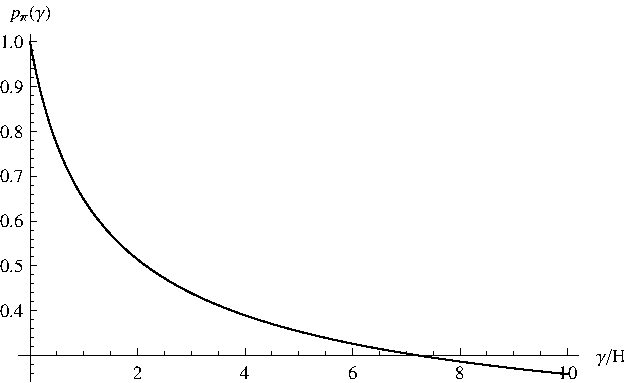
\includegraphics[width=8.5cm]{PowvsGamma}\par\smallskip
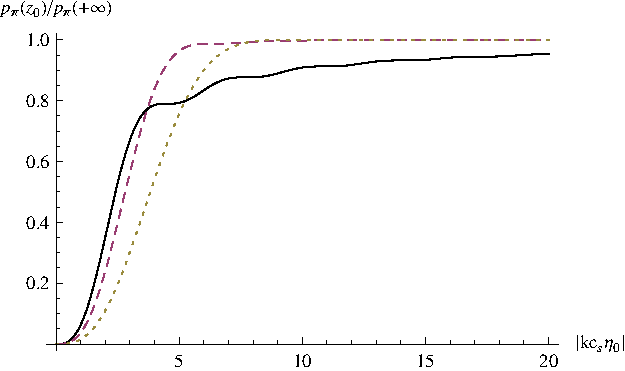
\includegraphics[width=8.5cm]{Powvsz0CG}
\caption{上：$z_0\to+\infty$における、式(\ref{pow1gamma})のパワースペクトルの$\gamma$依存性。$p_\pi(\gamma)=6N_c^2(kc_s)^3P_\pi(k)/(\pi\nu_{\calo})$と規格化した。下：$|kc_s\eta|\to0$におけるパワースペクトル$P_\pi(k)$の$z_0$依存性。$\gamma/H=0$（実線）、$\gamma/H=3$（破線）、$\gamma/H=9$（点線）を示す。}\label{casom}
\end{figure}

ADOFが（高い）温度$T$で熱平衡にあると仮定すると、FD定理から次が得られる。

\beq
\label{tempz}
k^3\langle\zeta_k\zeta_k\rangle_T \simeq  \sqrt{\pi\gamma_\star H_\star} \frac{TH_\star^2}{2c_s^\star\left({c^\star_s}^2N_c\right)}.
\eeq

これらは、数値因子を除けば式(\ref{tpnuo},\ref{tpwarm})の結果とまさに一致する。式(\ref{tempz})と類似した表式は文献\cite{berera1,berera2}で初めて導入され、温かいインフレーション模型\cite{warm}で重要な役割を果たす。

いくつか補足しておく。まず、一連の演算子を単一の演算子$\calo\pi$にまとめているため、扱う項の種類によって局所近似の見え方は大きく異なる。しかし、仮定を課した後の解析はかなり頑健であり、模型の細部には依存しない。保証する必要がある唯一の制約は2点関数のスケール不変性であり、これはインフレーション中に$\gamma,\nu_{\calo}$が比較的一定に保たれる限り保証される（詳細は後述する）。

非線形の次数に進むと、模型間の違いが役割を持ち始める。たとえば、摩擦項は演算子$\calo_\mu\delta g^{\mu0}$のみに由来するかもしれず、その場合は$\calo$と$\pi$の非線形結合を生じない。あるいは、スカラー結合$f(t)\calo$または$\calo\delta g^{00}$によって生じるかもしれず、その場合には互いにかなり異なる非線形相互作用が生じる。前述のとおり、$\calo\delta g^{00}$は最も明確な場合と考えられ、$f_{\rm NL}$の値が摩擦係数と結びつく。$f(t)\calo$では必ずしもそうならず、非Gaussian性の大きさは模型の詳細に依存する。しかし、前に論じたように、優先的な時計が1つだけ存在し、（非線形）応答$\delta\calo_R$が創発的シフト対称性を持つ場合には、$f_{\rm NL}$も同じように増大する。以下では、この解析をより精密にする。

\sectionlink{非Gaussian性}\label{nongaus}

本論文で論じた模型の非Gaussian的特徴は、観測的な特徴という観点からは、おそらく最も興味深い結果である。実際、2点関数は準de Sitter空間の対称性によって本質的に定まり、全体の振幅と傾きというわずか2つのパラメータで特徴づけられるのに対し、高次相関関数は関数としての自由度を持つ。それが観測されれば、それを生み出す物理機構について、はるかに多くの情報を読み解くことができる。

導入した広範な演算子のクラスについて非Gaussian的特徴を網羅的に調べることは、主としてその一般性ゆえに困難であり、本論文の範囲を超える。そこで、最低次の（スカラー）演算子$\calo\delta g^{00}$と$f(t)\calo$に注目する。非常に興味深いことに、対称性を課すことによって、運動方程式の線形寄与と非線形寄与の一部を関係づけられ、大きな散逸が大きな非Gaussian性と結びつくことを示す。続く各節では散逸が$\gamma\dot\pi$の形をとると仮定する。高階微分の散逸については\ref{localo2}節で調べる。

\subsectionlink{\texorpdfstring{$\calo\delta g^{00}$}{O δg⁰⁰}}\label{Nolocalo2}

ここでは、支配的な相互作用項が$\pi$の時間微分を1つ含み、$-\calo\delta g^{00}$という形のスカラー演算子によって生じる状況を解析する。この項には$\dot\pi$に線形な部分、より正確には$2\calo\dot\pi$が含まれる（以下では式(\ref{g00pi})による因子2を演算子$\calo$に吸収し、$\calo\to\calo/2$とする）。

ここでは、\ref{localapp}節で説明した局所近似について選択肢がある。すなわち、$\langle\delta\calo_S\delta\calo_S\rangle$と$G^{\calo}_{\rm ret}$に適用することも、$\langle\delta\dot\calo_S\delta\dot\calo_S\rangle$と$G^{\dot\calo}_{\rm ret}$に適用することもできる。前者の場合、通常の散逸項$\gamma\dot\pi$ではなく、ADL力に見られるような高階微分項が得られる。ここでは後者を解析し、前者は\ref{localo2}節で論じる。

$\delta\calo_S$の時間変化のスケールを$1/H$よりはるかに短いとするので、雑音への主な寄与は$\delta\dot\calo_S\gg H\delta\calo_S$から来る。すると、基本的には\ref{localapp}節と同じ手順により、線形次数での$\pi$の方程式が、式(\ref{fineom})で$\delta\calo_S$を$\delta\dot\calo_S$に置き換えたものに帰着することを示せる。パワースペクトルは、式(\ref{pow1gamma})において$\nu_{\calo}\to\nu_{\dot\calo}$と置き換えたもので与えられる。より明示的には、2次までの$\pi$の方程式は次となる。

\beq
\ddot\pi + 3H\dot\pi  - \frac{c_s^2\nabla^2}{a^2}\pi = -N^{-1}_c\left(\delta\dot{\calo} (1+\dot{\pi})+\delta\calo\ddot\pi -\frac{1}{a^2}\partial_i(\delta\calo\partial_i\pi)\right),\label{pieqnlprev}
\eeq

ここで$\delta\calo=\delta\calo_S+\delta\calo_R$である。式(\ref{g00pi})から、$\delta\calo$を擾乱する力は$F=\dot\pi+\dot\pi^2/2-(\partial_i\pi)^2/2$と分かる。ただし、\ref{localapp}節と同様に、応答部分の時間微分$\delta\dot\calo_R$に局所近似を用いると、次が得られる。

\beq
\label{ocaldot}
\delta\dot\calo_R\simeq N_c\gamma\left(\dot{\pi} +\frac{\dot{\pi}^2}{2}-\frac{\partial_i\pi\partial_i\pi}{2 a^2}\right).
\eeq

\ref{nonlineff}節ですでに述べたように、この局所近似だけでは、追加の仮定なしに非Gaussian性へのすべての寄与を計算することはできない。式(\ref{pieqnlprev})には$\delta\dot\calo$だけでなく$\delta\calo$も現れるためである。一般に、EFTの観点から精妙な相殺は予期されず、式(\ref{ratiogk})で見積もったように、非局所項の非Gaussian性への寄与は局所項の寄与と同程度と予想される。したがって以下では、$\dot\calo$のみを含む項に注目し、式(\ref{pieqnlprev})を次に簡約する。

\beq
\ddot\pi + (3H+\gamma)\dot\pi  - \frac{c_s^2\nabla^2}{a^2}\pi =\frac{\gamma}{2}\frac{\partial_i\pi\partial_i\pi}{a^2}-\frac{3\gamma}{2}\dot{\pi}^2 -N^{-1}_c\delta\dot{\calo}_S (1+\dot{\pi}).\label{pieqnl}
\eeq

まず右辺第1項$\gamma(\partial_i\pi)^2$の寄与に注目しよう。非Gaussian性を解析するため、$\pi=\pi_1+\pi_2$と分解する。添字は通常どおり、揺らぎに関する解の次数を表す。すると、

\be\label{pi1nl}\pi_1(k,\eta)=\frac{ k c_s}{N_cH^2}\int^{\eta}_{\eta_0} d\eta' g_{\gamma}(k c_s|\eta|,k c_s|\eta'|) \delta\dot{ \calo}_S,\ee

となる。ここで$g_{\gamma}(kc_s|\eta|,kc_s|\eta'|)=G_{\gamma}(kc_s|\eta|,kc_s|\eta'|)/(kc_s\eta')^2$であり、$G_{\gamma}$は式(\ref{greengamma})で定義される。また、式(\ref{pi1nl})を用いると、

\begin{eqnarray}
\pi_2(k_3,0)&=&\frac{\gamma k_3 c_s^3}{2 N_c^2H^4} \int^0_{\eta_0} d\eta' {\eta'}^2  g_{\gamma}(0,k_3c_s|\eta'|)\int\frac{d^3{\bf q}}{(2\pi)^3} |{\bf q}|  |{\bf k}_3-{\bf q}| ({\bf q}\cdot({\bf k}_3-{\bf q}))\nonumber\\
&\times&\int^{\eta'}_{\eta_0} d\eta'' g_{\gamma}(qc_s|\eta'|,qc_s|\eta''|) \int^{\eta'}_{\eta_0} d\eta''' g_{\gamma}(|{\bf k}_3-{\bf q}| c_s|\eta'|,|{\bf k}_3-{\bf q}| c_s|\eta'''|) \nonumber\\&\times&\delta\dot{\calo}_S({\bf q},\eta'')\delta\dot{\calo}_S({\bf k}_3-{\bf q},\eta''').\label{pi2nl}
\end{eqnarray}

となる（$\pi_2$の源は、摂動$\delta\dot\calo_S,\pi_1$について2次の項である）。

$\eta\to0$の極限における$\zeta\simeq-H\pi$の3点関数を計算したい。

\begin{eqnarray}\langle\zeta({\bf k}_1,0)\zeta({\bf k}_2,0)\zeta({\bf k}_3,0)\rangle&=&\langle\zeta_1({\bf k}_1,0)\zeta_1({\bf k}_2,0)\zeta_2({\bf k}_3,0)
\rangle+ \mbox{$k_i$の巡回置換の和}\nonumber\\
&\equiv&(2\pi)^3 \delta^{(3)}({\bf k}_1+{\bf k}_2+{\bf k}_3) F(k_1,k_2,k_3). \end{eqnarray}

式(\ref{twop1})、(\ref{twop2})と、雑音がGaussianであるという条件（非Gaussian雑音は後で考える）、すなわち

\begin{eqnarray}\label{os}&&\langle\delta\dot{ \calo}_S({\bf k}_2,\tilde{\eta'}) \delta\dot{\calo}_S({\bf k}_1,\tilde{\eta})  \delta\dot{\calo}_S({\bf q},\eta'')
\delta\dot{\calo}_S({\bf k}_3-{\bf q},\eta''')\rangle=(2\pi)^6\nu_{\dot{\calo}}^2\frac{\delta^{(3)}({\bf k}_1+{\bf k}_2+{\bf k}_3)}{a^4(\eta'')a^4(\eta''')}\\
&&\times \left\{\delta(\tilde{\eta'}-\eta'')\delta(\tilde{\eta}-\eta''')\delta^{(3)}({\bf k}_2+{\bf q})+
\delta(\tilde{\eta}-\eta'')\delta(\tilde{\eta'}-\eta''')\delta^{(3)}({\bf k}_1+{\bf q})\right\}\,\,\,(\mbox{ただし} \,\,\,k_3\neq 0)\nn,
\end{eqnarray}

を用い、任意の運動量スケール$k$に対して$x_i=k_i/k$と定義すると、$\eta_0\to-\infty$で次を得る。

\begin{eqnarray}\label{fdeltagooshape}
&&F(x_1,x_2,x_3)= k^6 F(k_1,k_2,k_3)=-\frac{\gamma H^3\nu_{\dot{\calo}}^2}{2N_c^4c_s^8}x_1^2x_2^2x_3(x_3^2-x_2^2-x_1^2)\int_{0}^{+\infty} dy y^2  g_{\gamma}(0,x_3 y)\\
&&\times\int_{y}^{+\infty} dz\,{z}^4 \,g_{\gamma}(x_2 y,x_2 z)  g_{\gamma}(0,x_2 z)\int_{y}^{+\infty} dw\,{w}^4 \,g_{\gamma}(x_1 y,x_1 w) g_{\gamma}(0,x_1 w)+\mbox{$x_i$の巡回置換の和}\nn
\end{eqnarray}

ここでは$y'=-kc_s\eta'$、$z=-kc_s\eta''$、$w=-kc_s\eta''$という変数変換を行った。

対応するパラメータ$f_{\rm NL}^{\rm eq}$（正三角形配置に対して定義する）は、次で与えられる。

\be F(1,1,1)=\frac{18}{5}f_{\rm NL}^{\rm eq}\Delta^2_{\zeta},\ee

ここで$\Delta_{\zeta}=k^3P_{\zeta}$である。Green関数を用いて表すと、

\begin{eqnarray}
f_{\rm NL}^{\rm eq}&=&\frac{5}{12}\left(\frac{\gamma}{Hc_s^2}\frac{2^{-8\gamma/H}\pi^2 {\Gamma\left(\frac{2\gamma}{H}+4\right)}^2}{\lp\frac{\gamma}{H}+1\rp^6{\Gamma\lp\frac{\gamma+H}{2 H}\rp}^8}\right)
 \int_{0}^{+\infty} dy {y}^2 g_{\gamma}(0, y)\int_{y}^{+\infty} dz z^4  g_{\gamma}( y,z)g_{\gamma}(0, z) \nonumber\\
&\times&\int_{y}^{+\infty} dw w^4  g_{\gamma}( y,w)g_{\gamma}(0, w),\label{fnlgoonoloc}
\end{eqnarray}

となる。ここでは式(\ref{pow1gamma})のパワースペクトルを、$\nu_{\calo}\to\nu_{\dot\calo}$として用いた。数値積分を行うと、

\beq
\label{fnlNL}
f_{\rm NL}^{\rm eq}\simeq-\frac{\gamma}{4H c_s^2},\eeq

が強散逸領域$\gamma\gg H$で得られる。$c_s\simeq1$であっても、これは大きくなりうる。文献\cite{Senatore:2009gt}の解析を用いると、桁の程度の上限も示すことができる。

\beq
\label{boundfnl}
\frac{\gamma}{H c_s^2} \lesssim 500.
\eeq

図\ref{shapegoonoloc}では、2つの$\gamma$の値（$\gamma=4H$および$40H$）について形状を描いた。正三角形配置にピークがあり、$x_2\simeq x_3\simeq1/2$の付近にも別のピークがあることに注意されたい。後者はバイスペクトルの主要な特徴の1つであり、揺らぎが雑音に支配されていることに由来する。

$\gamma\gg H$であってもその値が中程度の場合、形状は文献\cite{Senatore:2009gt}で述べられた直交型に似ている。この直交型は、現在のWMAP 7年データ\cite{Komatsu:2010fb}では$2\sigma$の水準にある。

\begin{figure}[htp]
\centering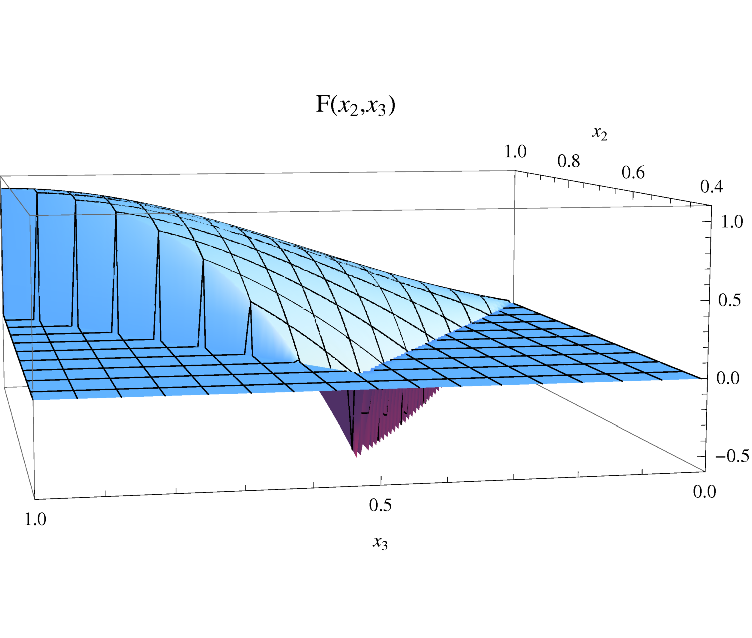
\includegraphics[width=8.5cm]{deltag00Noloc4}\par\smallskip
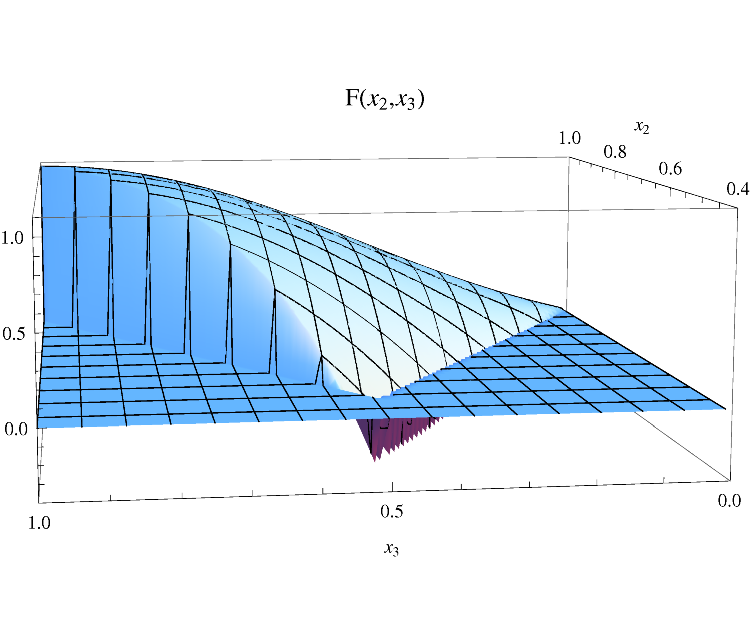
\includegraphics[width=8.5cm]{deltag00Noloc40}
\caption{式(\ref{fdeltagooshape})で与えられる形状$F(x_2,x_3)=x_2^2x_3^2\frac{F(1,x_2,x_3)}{F(1,1,1)}$。$\gamma=4H$（上）および$\gamma=40H$（下）の場合を示す。等価な配置の重複表示を避けるため、$1-x_2\leq x_3\leq x_2$の領域外では関数を0としている。}\label{shapegoonoloc}
\end{figure}

同様に、式(\ref{pieqnl})の右辺第2の源の項に対して、次を得る。

\begin{eqnarray}
f_{\rm NL}^{\rm eq}&=&-\frac{5}{2}\frac{\gamma}{H}\left(\frac{2^{-8\gamma/H}\pi^2 {\Gamma\left(\frac{2\gamma}{H}+4\right)}^2}{\lp\frac{\gamma}{H}+1\rp^6{\Gamma\lp\frac{\gamma+H}{2 H}\rp}^8}\right)
 \int_{0}^{+\infty} dy  g_{\gamma}(0, y)\int_{y}^{+\infty} dz z^4  y\frac{d g_{\gamma}}{dy}( y,z)g_{\gamma}(0, z) \nonumber\\
&\times&\int_{y}^{+\infty} dw w^4  y\frac{dg_{\gamma}}{dy}(y,w)g_{\gamma}(0, w).\label{fnlgoonolocdot1}
\end{eqnarray}

見かけによらず、この項の$f_{\rm NL}^{\rm eq}$への寄与は$\gamma$とともに増大せず、1の程度の副次的な効果となる。これはGreen関数の性質から従い、特に時間微分が$\sqrt{\gamma H}$ではなく$H$のべきでスケールすることによる。凍結時のGreen関数がそのような時間依存性を持つためである。これは、\ref{noise}節の平坦時空での結果（「$\tau_{\rm eq}$」$\sim1/H$）からまさに予想されることである。これらのGreen関数に関する詳細のまとめは付録\ref{greenf}を参照されたい。

式(\ref{pieqnl})の最後の項については、次が得られる。

\begin{eqnarray}\label{fnlOdotpi}
f_{\rm NL}^{\rm eq}&=&\frac{5}{3}\left(\frac{2^{-8\gamma/H}\pi^2 {\Gamma\left(\frac{2\gamma}{H}+4\right)}^2}{\lp\frac{\gamma}{H}+1\rp^6{\Gamma\lp\frac{\gamma+H}{2 H}\rp}^8}\right)
 \int_{0}^{+\infty} dy  y^4\, (g_{\gamma}(0, y))^2\int_{y}^{+\infty} dz z^4  y\frac{d g_{\gamma}}{dy}(y,z)g_{\gamma}(0, z),\label{fnlgoonolocdot2}
\end{eqnarray}

これも1の程度の寄与であり、$\gamma$とともに増大しない。この項に対応する形状を、$\gamma=10H$の場合について図\ref{ngg10}に示す。

予想どおり、これらの形状はすべてスクイーズド極限に近づくと抑制される。寄与が$\pi$の時間微分を含み、また$\delta{\cal O}$が局所的だからである。この極限とは、運動量の1つ、たとえば$k_1\equiv k_L$（長波長モード）が、他の2つ（短波長モード）よりはるかに小さい場合、すなわち$k_L\ll k_S$（$k_S=|{\bf k}_2-{\bf k}_3|/2$）である。ただし、興味深い問題が残る。それは、この抑制が局所型の形状と比べて$k_L$の1乗、あるいはそれ以上のべきを伴うかどうかである。この特定のスケーリングにより、スケール依存バイアスの測定において単一場模型の特徴を識別できる可能性があるためである\cite{creminelli11}。この点には次節で戻る（図\ref{ngg10}から、形状そのものがスクイーズド極限$k_L/k_S\to0$で0に近づくことを指摘しておく。したがって$F(x_1,x_2,x_3)$は$1/x_L^2\equiv(k_S/k_L)^2$のようにはスケールせず、それより弱いべきで振る舞う）。

\begin{figure}[htp]
\centering
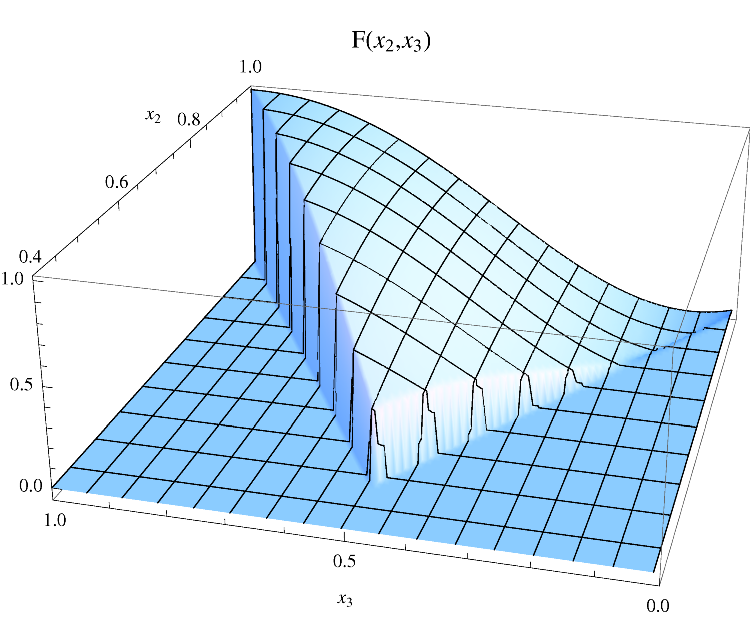
\includegraphics[width=8.5cm]{NGGamaOdotpigamma10}
\caption{式(\ref{pieqnl})の最後の項に対応する、$\gamma=10H$の場合の形状$F(x_2,x_3)=x_2^2x_3^2\frac{F(1,x_2,x_3)}{F(1,1,1)}$。}\label{ngg10}
\end{figure}

\subsectionlink{\texorpdfstring{$f(t)\calo$ I：線形応答}{f(t)O I：線形応答}}\label{ftcalo}

今度は、式(\ref{inter1n})にあるような$f(t)\calo$の形の相互作用による寄与を考えよう。可能性を線形応答と非線形応答の2つに分け、後者は次節で扱う。

線形応答理論で非線形効果を計算するため、ADOFに作用する力を$\pi$の2次まで用いる。これは$F=\dot f\pi+\ddot f\pi^2/2+\ldots$で与えられ、省略記号は$f(t)$の高階時間微分に比例する、$\pi$のより高いべきの項を表す。\ref{appsh}節で述べたように、一般にはスローロール近似でこれらの項を無視する。したがって以下では、$\dot f$を本質的に一定として扱う。

$G_{\rm ret}^{\calo}$の局所近似のもとで、応答部分$\delta\calo_R$は次のように書ける。

\be
\label{ddff}
\delta\calo_R\simeq \frac{\gamma N_c}{\dot{f}}\left(\dot{\pi}+\frac{\ddot{f}}{\dot{f}}\dot{\pi}\pi\right),
\ee

ここでは、スローロールパラメータのより高いべきで抑制される項を除いた（微分を含まない項を無視するため、創発的シフト対称性の存在を仮定していることを思い出されたい）。したがって、$\pi$の2次までの方程式は次となる。

\be\label{pia}
\ddot{\pi}+(3H+\gamma)\dot{\pi}+\frac{k^2c_s^2}{a^2}\pi+2\gamma\frac{\ddot{f}}{\dot{f}}[\pi\dot{\pi}]_k=-N_c^{-1}\left(\dot f\delta \calo_S+\ddot{f}[\pi\delta \calo_S]_k\right),
\ee

ここで雑音部分$\delta\calo_S$は式(\ref{twop1},\ref{twop2})を満たす。この方程式を式(\ref{fineom})と比較すると、パワースペクトルは全体の因子$\dot f^2$を除いて式(\ref{pow1gamma})と同じである。すなわち、$\nu_{\calo}\to\nu_{f\calo}=\dot f^2\nu_{\calo}$とすればよい。したがって、パワースペクトルのスケール不変性を保証するには、$\dot\nu_{f\calo}/(\nu_{f\calo}H)\simeq O(\epsilon)$が必要である（これについては後で詳しく述べる）。

\ref{appsh}節で強調したように、上の非線形項による$f_{\rm NL}$への寄与は$\ddot f/(\dot fH)\simeq O(\epsilon)$で抑制される。この次数では、重力との混合などの他の効果をもはや無視できないことに注意されたい。さらに、次節で非Gaussian性が非線形応答によって支配されることを示す。それでもここに式(\ref{pia})の項の計算を含めるのは、2つの理由による。まず、非線形項は$\gamma$に比例していても、最終的な答えではその因子が消えることを明示するためである。より重要なのは、$\dot f$が定数でない場合、スクイーズド極限で無視できないかもしれない寄与を与えるように見えるためである。

まず式(\ref{pia})の最後の源の項$\ddot f\pi\delta\calo_S$を解析しよう。この項は$\pi$の微分を十分には含まないため、$F(x_2,x_3)=x_2^2x_3^2\frac{F(1,x_2,x_3)}{F(1,1,1)}$で与えられる形状の寄与がスクイーズド極限で最大となることは容易に分かる。その極限では、パラメータ$f_{\rm NL}$は次で与えられる。

\begin{equation}\label{squ}
f_{\rm NL}^{\rm sq} =\lim_{x_3\to 0,\,\ x_2\to 1}\frac{5}{6} \frac{F(1,x_2,x_3)}{(P_{\zeta}(1)P_{\zeta}(x_2)+P_{\zeta}(1)P_{\zeta}(x_3)+P_{\zeta}(x_2)P_{\zeta}(x_3))}.
\end{equation}

前節までと同様の手順に従うと、次を得る。

\beq f_{\rm NL}^{\rm sq}\simeq-\frac{5 }{6}\frac{\ddot{f}}{H\dot{f}} \label{fnlddf},\eeq

これは$\gamma$の値によらない。式(\ref{estfto})の先の見積もりと一致する。同様に、式(\ref{pia})の左辺最後の項の寄与も計算できる。この項は$\gamma$に比例するが、パラメータ$f_{\rm NL}$は上の値に比べて顕著には増大しない。これは\ref{appsh}節の発見的議論から従うが、Green関数の性質から直接見ることもできる。付録\ref{greenf}を参照されたい。近似的シフト対称性が$\ddot f/(H\dot f)\simeq O(\epsilon)$を要請するため、前述のとおり式(\ref{fnlddf})の$f_{\rm NL}^{\rm sq}$は非常に小さくなる。

それでも、パワースペクトルに現れる組み合わせ$\nu_{f\calo}=\dot f^2\nu_{\calo}$を一定に保つ一方で、$\dot f,\nu_{\calo}$は近似的に一定でないと仮定した場合、式(\ref{fnlddf})の結果が気になるかもしれない。しかし上の計算は不完全である。非線形の次数では、$\pi$が雑音の確率密度汎関数にも影響することによる寄与があるためである（これらは$\dot\nu_{\calo}\ll H\nu_{\calo}$の極限で抑制される）。すべての寄与を考慮すれば、地平線の外に時計以外のいかなる摂動も含めていないという事実と整合するために、最終的には$f_{\rm NL}^{\rm sq}$は$(n_s-1)$に比例するはずである\cite{consist,Cheung:2007sv}。

スクイーズド極限の性質をよりよく理解するために、本研究でよく現れる$\delta\calo\dot\pi$型と$\delta\calo\pi$型の非線形性の寄与を比較しよう。両者で$\calo$演算子を同じものに固定すると、重要な違いは、後者の形状が$g_\gamma(x_Ly,z)$を含むのに対し、前者は$y\partial_yg_\gamma(x_Ly,z)$を含むことであると容易に分かる（$z,y$は積分変数）。次を用いると、

\beq
\frac{y\partial_{y}g_{\gamma}(x_L y, z)}{  g_{\gamma}(x_L y, z)}\sim \frac{x_L^2y^2}{(1+\gamma/H)},
\eeq

これは$yx_L\ll1$で成り立ち、積分が$\sqrt{\gamma/H}$付近の$y,z$の値に支配されること（付録\ref{greenf}参照）も考慮して、$x_L^2\ll H/\gamma$の領域では、$\delta\calo\dot\pi$のスクイーズド極限は$\delta\calo\pi$の寄与に比べて$x_L^2=(k_L/k_S)^2$の因子で抑制されると結論できる。これは文献\cite{creminelli11}の結果と一致する。スクイーズド極限と整合性条件については、別の機会により詳しく議論する。

次に、非Gaussian性への最大の寄与を与えることになる$f(t)\calo$結合の非線形応答を調べる。

\subsectionlink{\texorpdfstring{$f(t)\calo$ II：非線形応答}{f(t)O II：非線形応答}}\label{nonlrep}

これまでは、応答$\delta\calo_R$を$\pi$の線形次数で考えてきた。そのために必要なのは2点関数$G_{\rm ret}^{\calo}$のみである（式(\ref{gnoa1})参照）。しかし、$\delta\calo$の高次の$n$点関数へ進むことによっても非線形性を誘起できる。たとえば、その3点関数

\beq
C^{\calo}_{\rm ret} (x,y,z) \equiv \langle [\delta\calo(z),[\delta\calo(y),\delta\calo(x)]]\rangle \theta(t_y-t_z)\theta(t_x-t_y),
\eeq

を含め、力は最低次の$F(\pi)=\dot f\pi$のままにする（以下では$\dot f$を定数として扱う）。すると、

\beq
\label{calo12}
\dot f \delta\calo_R(x) = -\dot f^2 \int G^\calo_{\rm ret}\pi(y) dy + \dot f^3 \int dydz~C^{\calo}_{\rm ret}(x,y,z)\pi(y)\pi(z) + \ldots
\eeq

となる。省略記号は高次の補正を表す。

先験的には、両者が空間と時間について局所的であると仮定しても、$G_{\rm ret}^{\calo}$と$C_{\rm ret}^{\calo}$の間に関係は期待されない。しかし、以下で論じるように、ADOFの応答が単一の（優先される）時計によって支配される場合には、両者の関係が得られる。

本論文を通して強調したように、演算子$f(t)\calo$から散逸項を得るためには、局所的なGreen関数を仮定すると、次が必要である。

\beq
\dot f  \delta^{(1)}\calo_R = N_c \gamma \dot\pi.
\eeq

この式は示唆的な形に次のように書き換えられる。

\beq
\label{onecalR}
\dot f  \delta^{(1)}\calo_R = N_c \gamma~\delta^{(1)}\left\{n^\mu\partial_\mu(t+\pi)\right\},
\eeq

ここで（$O(\pi^2)$を除いて$n^0=1$であることに注意されたい）、

\beq
\label{nmu2} n^{\mu}=\frac{-g^{\mu\nu}\partial_{\nu}{\tilde t}}{\sqrt{-g^{\nu\rho}\partial_{\nu}{\tilde t}\partial_{\rho}{\tilde t}}},
~~\tilde t = t+\pi, \eeq

とする。これにより、式(\ref{onecalR})は$\calo$がスカラー演算子であるという対称性を明示する。すると、応答を$\pi$の全次数に外挿でき、次が得られる。\footnote{原理的には、これは$F_\calo\left(\sqrt{-g^{\nu\rho}\partial_\nu\tilde t\partial_\rho\tilde t}\right)$へ一般化できる。簡単のため、$F_\calo(x)=x$に限定する。}

\beq
\label{gretto2p}
\dot f  \delta^{(n)}\calo_R = N_c \gamma~\delta^{(n)}\left\{n^\mu\partial_\mu(t+\pi)\right\} = N_c\gamma~\delta^{(n)}\left(\sqrt{-g^{\nu\rho}\partial_{\nu}{\tilde t}\partial_{\rho}{\tilde t}}\right).
\eeq

この式が、運動方程式における線形項と非線形項の関係を意味することは容易に示せる。たとえばユニタリーゲージ、すなわち$\tilde t=t$では、

\beq
\label{dpcalfn}
\dot f  \delta^{(n)}\calo_R = N_c \gamma~\delta^{(n)}\sqrt{-g^{00}},
\eeq

となり、$g^{00}(\pi)=-1-2\dot\pi-\dot\pi^2+(\partial_i\pi)^2$を用いて$\pi$の相互作用を読み取れる。したがって、

\bea
-\dot f \delta^{(1)}\calo_R &=& -N_c \gamma \dot\pi,\\
-\dot f \delta^{(2)}\calo_R &=& \frac{1}{2} N_c \gamma (\partial_i\pi)^2 
\label{dpcalo2}.
\eea

となる。こうして、厳密なシフト対称性の場合に得られたものと似た非線形項が得られる（式(\ref{pieqnl})の右辺第1項を参照し、式(\ref{ocaldot})とも比較されたい）。\footnote{式(\ref{dpcalfn})の型の非線形応答では$\dot\pi^2$項が得られなかったことに注意されたい。しかし、一般的な関数$F_\calo(\sqrt{-g^{00}})$を許せば、この項も生じうる。}非Gaussian性の解析は\ref{Nolocalo2}節と同様に進み（\ref{shsym}節も参照）、

\beq
f_{\rm NL} \simeq -\frac{\gamma}{c_s^2 H},
\eeq

となる。これは\ref{nlrep}節で予想したとおりである。形状も図\ref{shapegoonoloc}に似たものとなる。

前の議論は、従来のスカラー場インフレーション模型に限定すると、より分かりやすいかもしれない。重要な点は、摂動への応答が微分同相不変性と整合しなければならないことである。そのため散逸を誘起するには$\dot\phi$の因子が必要であり、それがさらに、\ref{nlrep}節で概略を述べたように、$\gamma\gg H$の場合に大きな非Gaussian性をもたらす。

論理は次のとおりである。$\calo$をスカラー演算子として、次の形の相互作用Hamiltonianを考えよう。

\beq
H_{\rm int} = \phi\; \calo \label{hint}.
\eeq

インフラトンの運動方程式は、したがって次となる。

\beq
\label{eomphi}
D_\phi \phi = \calo,
\eeq

ここで$D_\phi\phi=0$は$\calo$が存在しない場合の運動方程式を表す。もちろん、$\calo$の背後には独自の$\calL_\calo$を持つ力学系がある。しかし、EFTの考え方に従い、式(\ref{hint})の結合以外は何も仮定しない。まず背景$\bphi(t)$を求めることから始める。局所的な応答を仮定すると、

\beq
\label{gcalo}
\langle \bphi|\calo |\bphi\rangle = F_\calo(\bphi, \dot{\bphi}),
\eeq

となる。括弧は、$\bphi$が与える背景で応答を計算していることを強調する。式(\ref{eomphi})に代入すると、次を得る。

\beq
\label{dphibpi}
D_\phi \bphi = F_\calo(\bphi, \dot{\bphi}).
\eeq

本論文で調べる型の、速度に依存する散逸を得るため、次を課す。

\beq
\label{fphip}
 F_\calo(\bphi, \dot{\bphi})\simeq |\dot\bphi|.
\eeq

この振る舞いの具体例を、より複雑な応答関数を用いてではあるが、\ref{matching}節で論じる。次の段階は$\bphi\to\bphi+\delta\phi$という摂動を加えることである。議論の要点は、式(\ref{gcalo})を何が置き換えるかにある。この問題に取り組む方法はいくつかあるが、おそらく最も簡単なのは次の方法である。$\calo$は構成上スカラー演算子なので、式(\ref{gcalo})を共変化しなければならない（Lorentz不変性は、優先される基準系の存在、すなわち式(\ref{nmu2})で$\tilde t$を$\phi$に置き換えた$n^\mu$によってのみ破られる）。したがって、先の議論のとおり、式(\ref{gcalo})を次のように書き換えるべきである。

\beq
\label{gcalo2}
\langle \phi|\calo |\phi\rangle = F_\calo\left(\phi, n^\mu \partial_\mu \phi = -g^{\mu\nu}\partial_\nu\phi\partial_\mu\phi/\sqrt{-g^{\mu\nu}\partial_\nu\phi\partial_\mu\phi}\right),
\eeq

ここでは関数$F_\calo$が本質的には変化しないと仮定した。これは$\delta\phi$が滑らかな長波長摂動であれば妥当な局所近似である。\footnote{言い換えると、明確に定義された微分展開を持つために、等時刻面の外部曲率の変化スケール（$K^{ij}\simeq\nabla^i_{(3)}n^j$に注意）が、$\phi$と$\calo$の相互作用の局所近似を支配する典型的長さスケール$M_\calo^{-1}$よりはるかに大きい必要がある。たとえば地平線通過時の摂動$\delta\phi_{k_\star}$をとり、$g$を結合定数として$M_\calo^2\simeq g|\dot\bphi|$とすれば、$k_\star^2\ll M_\calo^2$、あるいは$\gamma<g|\dot\bphi|/H$が必要である（完全に一般的には、抑制されていても$\delta K_{\mu\nu}$による補正も原理的には含めるべきである）。詳細は\ref{localtrap}節を参照されたい。}

再びユニタリーゲージに移り、$\phi=\bphi$、すなわち$\delta\phi=0$となる座標を選ぶ。これは次を意味する。

\beq
\label{gcalo3}
\langle \phi| \calo |\phi \rangle = F_\calo\left(\bphi,\dot\bphi\sqrt{-g^{00}}\right).
\eeq

次に、式(\ref{dphibpi})とSt\"uckelbergの方法を用いて摂動$\delta\phi$（ここでの$\pi$）を導入する。左辺には通常の項が得られ、右辺には式(\ref{fphip})の要請を用いると、

\beq
D_\phi \delta\phi  \simeq \delta \left(|\dot\bphi| \sqrt{-g^{00}(\pi)}\right),
\eeq

となる。これは式(\ref{dpcalfn})から得られた結果に似ており、$\pi=\delta\phi/\dot\bphi$である。そして前述のとおり、散逸項$\gamma\dot\pi$に加えて$\gamma(\partial_i\pi)^2$も得られ、\ref{Nolocalo2}節で示したように、これによって非Gaussian性が増大する。

前の議論には、強調しておくべき微妙な点がある。厳密には、散逸の存在が要求するのは$\pi$への線形結合のみである。我々の議論で式(\ref{gretto2p})の$n^\mu\partial_\mu\pi$から得られた非線形項は、$n^\mu$が、インフレーションの終了を制御する物理的時計の一様なスライスに直交する時間的ベクトルであることと本質的に結びついていた。しかし一般には、ADOFに時間的ベクトル演算子が含まれることもあり、これらをまとめて$u_\calo^\mu$と書くと、背景で非ゼロの期待値を持ちうる。したがって、式(\ref{gretto2p})には$n^\mu\partial_\mu\pi$に代わって$u_\calo^\nu\partial_\nu\pi$が現れるかもしれない。\footnote{これは、$\calo$の応答が$u_\calo^\mu$によって制御される場合に起こりうる。}その場合、線形項$\gamma\dot\pi$（今度は$\langle u_\calo^\mu\rangle=(1,0,0,0)$から導かれる）と、その非線形の対応物との関係は保証されない。この状況では、大きな散逸が必ずしも強い非Gaussian性をもたらすとは限らない。

\ref{newdof}節で導入したGoldstoneボソン$\tilde\pi$を直接用いることを選んでいれば、非ゼロの期待値をとるベクトル型演算子は存在しなかったはずである。この場合、背景の期待値を持つ唯一のベクトルは、規格化を除けば$n^\mu\sim g^{\mu\nu}\partial_\nu(t+\tilde\pi)$となり、式(\ref{dpcalo2})の型の項を誘起するように見える。しかし2つの記述は等価である。実際、模式的に$\tilde\pi\sim\pi+\delta O$であることに注意すると、この場合であっても、$\tilde\pi$とベクトル演算子の揺らぎ$\delta u_\mu^\calo$の相互作用により、非線形次数で式(\ref{dpcalo2})の項が生成されなくなる可能性を一般には排除できない。したがって、散逸と非Gaussian性との関係を保証するために、そのような相殺がないことを要請する。

この条件を実装する簡単な方法はない。ただし実際には、$\delta\calo$が、その揺らぎによってインフレーションの終了を制御する場$\pi$に主として感度を持つことを要請することに相当する。本論文では、この条件を「優先的な時計を持つ」と表現してきた。

したがって、そのような時計の存在は、強散逸領域において必然的に大きな非Gaussian性を伴うと結論できる。それは\ref{Nolocalo2}節で明示した$\calo g^{00}$に由来する場合も、今説明した$f(t)\calo$の非線形応答を通じて生じる場合もある。この仮定を緩めることについては今後の研究で扱う。

\subsectionlink{非Gaussian雑音}\label{ngaussnoise}

非Gaussian性の最後の源として、雑音揺らぎに内在する非Gaussian性の効果を考える必要がある。式(\ref{ngnoise})と同様に、局所的な非Gaussian雑音$\delta\calo_S$を考えよう。すなわち、

\beq
\langle\delta\calo_S(t_1, {\bf k}_1)\delta\calo_S(t_2, {\bf k}_2)\delta\calo_S(t_3, {\bf k}_3)\rangle\simeq (2\pi)^3\delta^{(3)}({ \bf k}_1+ {\bf k}_2+ {\bf k}_3)\nu_{{\calo}^3}\frac{\delta(t_1-t_2)}{a^{3}(t_1)}\frac{\delta(t_2-t_3)}{a^3(t_2)}.
\eeq

である。次を用いると、

\beq \pi(t, {\bf k})=\frac{\dot{f} k c_s}{N_c H^2}\int^{\eta}_{\eta_0} d\eta' g_{\gamma}(kc_s |\eta|, k c_s|\eta'|)\delta\calo_S(\eta',{\bf k})
\eeq

$\eta\to0$かつ$\eta_0\to-\infty$に対して、次を得る。

\beq\label{NGNoise}
F(x_1,x_2,x_3)=-\frac{\dot{f}^3 H^5\nu_{{\calo}^3}}{N_c^3c_s^6}x_1x_2x_3\int_0^{+\infty} dz z^8 g_{\gamma}(0,x_1 z)g_{\gamma}(0,x_2 z)g_{\gamma}(0,x_3 z).\eeq

\begin{figure}[h!]
\centering
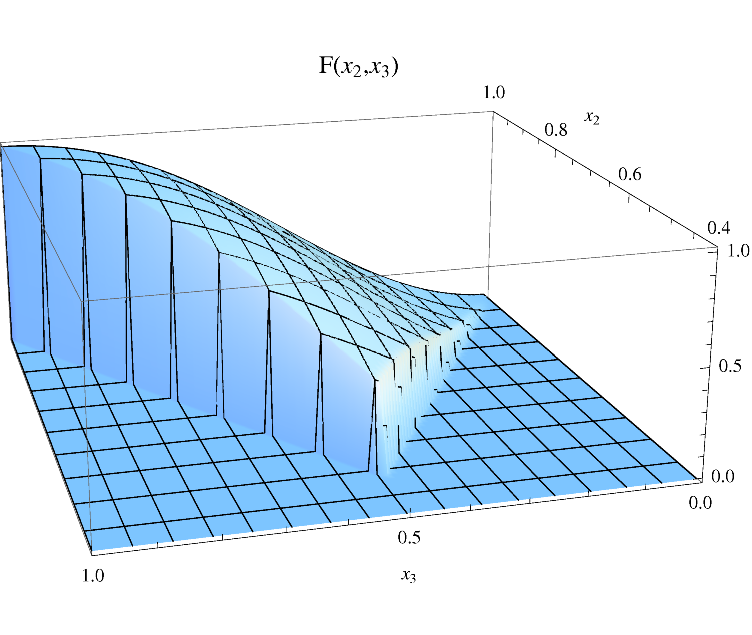
\includegraphics[width=8.5cm]{NGCG10Noise}
\caption{式(\ref{NGNoise})から得られる、$\gamma\simeq10H$の場合の形状$F(x_2,x_3)=x_2^2x_3^2\frac{F(1,x_2,x_3)}{F(1,1,1)}$。等価な配置の重複表示を避けるため、$1-x_2\leq x_3\leq x_2$の領域外では関数を0としている。}\label{nonGausNoise}
\end{figure}

形状を図\ref{nonGausNoise}に示す。予想どおり正三角形配置にピークがあり、

\beq
f_{\rm NL}^{\rm eq}\simeq \frac{\gamma N_c\nu_{{\calo}^3} }{\dot{f} \nu_{\calo}^2},
\eeq

となる。これは式(\ref{fnlnoise})で予想したとおりである。

\subsectionlink{高階微分の散逸}\label{localo2}

今度は\ref{Nolocalo2}節と同じく、支配的な相互作用$\delta g^{00}\calo$が$\pi$の微分を1つ含む状況を考えよう。ただし、前とは異なり、ここでは$\calo$の2点関数に局所近似（あるいは${\rm Im}G_{\rm ret}^{\calo}\sim\omega$）を仮定する。その結果、次が得られる。

\beq\label{eq:help}\delta\calo_R\simeq-\frac{N_c}{a^3\Gamma_\calo}\partial_t(a^3\dot{\pi}),\ee

ここで$\Gamma_\calo$は質量の次元を持ち、模型の具体的な詳細に依存する。相互作用項が$\pi\delta\dot\calo$の形であることから、運動方程式は次となる。\footnote{$H/\Gamma_\calo$の程度の音速の補正も生じるが、ここでは無視する。}

\beq \ddot{\pi}+\frac{c_s^2k^2}{a^2}\pi+3H\dot\pi- \frac{1}{\Gamma_\calo a^3}\partial_t^2(a^3\dot\pi)=-\frac{\partial_t(a^3\delta\calo_S)}{a^3N_c},\eeq

この方程式はADL力を思わせるものになっている。高階微分項の存在によって、$\omega\simeq H\ll\Gamma_\calo$に制限し、高階微分項を小さな摂動として扱わなければならない。この場合、凍結は$\omega\sim H$で起こり、主要な効果は、ここでは真空解に支配される2点関数ではなく、3点関数に現れる。これは、運動方程式の非線形項を線形項と比較することで見積もれる。2次の方程式は次のように書ける。

\be\ddot{\pi}_2+\frac{{c}_s^2k^2}{a^2}\pi_2+H\lp3+\frac{ k^2c_s^2 \delta}{a^2H^2}\rp\dot{\pi}_2=J_k,\ee

ここで$J_k$は2次の源を含む。$\pi$と$\delta\calo$の結合から、次が得られる。

\be \label{source}J_k=-\frac{1}{N_c}\left\{\frac{\partial_t(a^3{\delta}_2\calo)}{a^3}+\frac{\partial_t(a^3\dot{\pi}_1{\delta}_1\calo)}{a^3}-\frac{\partial_i({\delta}_1\calo\partial_i\pi)}{a^2}\right\},\ee

ここで$\delta\calo=\delta\calo_S+\delta\calo_R$であり、添字は寄与を$\pi$の何次まで計算するかを表す。見積もりのため、音速が小さい模型で支配的となる最後の項を考える。式(\ref{eq:help})を用いると、非Gaussian性の大きさは次で与えられる。

\be
f_{\rm NL}\zeta\sim\left.\frac{\frac{1}{N_c}\partial_i({\delta}_1\calo\partial_i\pi)}{\ddot\pi}\right|_{\omega\sim H}\sim\frac{H^4 \pi^2}{c_s^2 \Gamma_\calo}\cdot \frac{1}{ H^2\pi}\sim\frac{H}{\Gamma_\calo}\cdot\frac{1}{c_s^2}\zeta\ll \frac{1}{c_s^2}\zeta,
\ee

したがって、これは高々副次的な信号にしかなりえない。

\sectionlink{インフレーション中の散逸効果のマッチング}\label{matching}

EFTの立場では$G_{\rm ret}^{\calo}$と雑音核に対する条件を与えられたものとして扱えるが、それでも、これらの条件がある程度の近似で確かに成立する状況を特定できることが望ましい。たとえば、式(\ref{drude})のDrude模型のように、記憶効果が十分速く減衰する場合には、この記述が有効であると予想される。これは、短い相互作用時間の後に$\pi$場への逆反応が無視できるような$\calo$の力学であれば成り立つ。本節では、文献\cite{trapped}のトラップ型インフレーション模型の考え方に沿った具体的実現を調べ、温かいインフレーションの枠組み\cite{berera1,berera2,warm}についても簡単に論じる。$\calo\dot\pi$結合によって$\gamma\dot\pi$の散逸を生じる模型のクラスについては、付録\ref{mag00}を参照されたい。

\subsectionlink{\texorpdfstring{局所的なトラップ型インフレーション：$f(t)\calo\to\sum_i(\phi-\phi_i)^2\chi_i^2+\calL(\chi_i)$}{局所的なトラップ型インフレーション：f(t)O → Σᵢ(φ−φᵢ)²χᵢ² + L(χᵢ)}}\label{localtrap}

時間に関する局所近似を適用できる例を求めたい。トラップ型インフレーションでは、粒子が生成されることと、その質量が時間とともに増大することの両方によって、インフラトンのエネルギーがADOFに移される。元の模型では、宇宙膨張によって粒子が十分に希釈されるまで、これが重要である。そのための特徴的時間スケールは$H^{-1}$であり、これまで用いてきた局所的応答関数を使うことはできない。しかし、生成粒子がさらに別の自由度へ、Hubbleよりはるかに速い崩壊率で崩壊すれば、この特徴的時間スケールを大幅に短くできる。この点を念頭に置いて、トラップ型インフレーションの作用を考えよう。

\beq \label{seftrap} S_{\rm trap}=\int d^4x\sqrt{-g} \left\{\sum_i\left[-\frac{1}{2}\partial_{\mu}\chi_i\partial^{\mu}\chi_i-\frac{ g^2(\phi-\phi_i)^2}{2}\chi_i^2\right]-\frac{1}{2}\partial_{\mu}\phi\partial^{\mu}\phi-V(\phi)\right\},\eeq

ここで$\phi$はインフラトン、$V(\phi)$はそのポテンシャルである。さらに、$\chi_i$と追加の自由度$\varphi$との結合を特徴づける相互作用項$S_{\rm int}(\chi_i,\varphi)$を加える。この結合による$\chi_i$の崩壊率は$\Gamma_{\chi_i}\gg H$を満たすものとする。課す必要のある唯一の条件は、$S_{\rm int}$が$S_{\rm trap}$から得られる最低次の描像を変えないことである。特に、$\phi\simeq\phi_i$のときに$\chi_i$に大きな質量を生じないことを保証する必要がある。たとえば、次の形が考えられる。

\beq
\label{decayr}
S_{\rm int} =  \sum_i \frac{1}{\Lambda_\varphi} \partial^2\chi_i \varphi^2,
\eeq

ここで$\varphi$はスカラー場であり、小さな質量$m_\varphi\lesssim\sqrt{g|\dot\phi|}$を持ち、$\phi$とは直接結合しないと仮定する。以下では、この模型で局所近似が可能であることを示す（本節では表記を簡単にするため、$\phi$の非摂動値を示す上線を省く）。

元のトラップ型インフレーションのシナリオと同様に、$\phi$が$\phi_i$に近づくと、場$\chi_i$に対応する粒子が生成される。粒子生成の計算は文献\cite{trapped,beauty}と同じ方針で進める。ある$\chi_i$場のモードが断熱的に振る舞わず、対応する粒子が生成される時間間隔$\delta t_c=t-t_i$は、次のように見積もれる。

\be \delta t_c\sim 1/\sqrt{g|\dot{\phi}|},\ee

これをHubble時間より短く、$\delta t_c\ll H^{-1}$としたいので、次が必要である\cite{trapped}。

\be\label{c1}
H^2\ll{g|\dot{\phi}|}.
\ee

この条件は、粒子生成後の質量が次を満たすことを意味する。

\be M_{\chi_i}(t_i+\delta t_c)=g|\phi-\phi_i|\simeq g|\dot{\phi}|\delta t_c\gg H.
\ee

次に崩壊率について、式(\ref{decayr})を用いると、次のように見積もれる。

\beq
\Gamma_{\chi_i} \simeq  \frac{M_{\chi_i}^3}{\Lambda_\varphi^2}. \label{gammab}
\eeq

崩壊の時間スケールが粒子生成に要する時間より長いことを保証するには、次が必要である。

\beq
\label{c2n}
 \frac{1}{\delta t_c}\simeq \sqrt{g|\dot\phi|}\gtrsim \Gamma_{\chi_i}\simeq\frac{(g|\dot{\phi}|)^{3/4}}{ \Lambda_\varphi^{1/2}} \quad\to\quad  \Lambda_\varphi \gtrsim \sqrt{g|\dot\phi|},
\eeq

ここでは$\chi_i$粒子の寿命を$\tau_{\chi_i}$として、$M_{\chi_i}\simeq g|\dot\phi|\tau_{\chi_i}\equiv M_{\chi_i}(\tau_{\chi_i})$と近似した。同時に、局所近似に必要な$\Gamma_{\chi_i}\gg H$も成り立つ。\footnote{$\tau_{\chi_i}>\delta t_c$は$\Gamma_{\chi_i}<M_{\chi_i}(\tau_{\chi_i})$を要求し、これは粒子としての解釈とも整合することに注意されたい。}粒子が生成された後、各粒子種の占有数は次で与えられる。

\beq
\label{ocupnum}
|\beta_k|^2=e^{-\frac{\pi k^2}{a^2(t_i)\kappa^2(t_i)}},
\eeq

ここで$\kappa(t_i)=\sqrt{g|\dot\phi(t_i)|}$であり、数密度は

\be\label{nchim} n_{\chi_i}(t_i+\delta t_c)=M_{\chi_i}\bar\chi^2_i\simeq \frac{\kappa^3(t_i)}{(2\pi)^3}.\ee

となる。その後の時刻では粒子の崩壊率を考慮して、

\be n_{\chi_i}(t,t_i)\simeq \frac{\kappa^3(t_i)}{(2\pi)^3}\lp\frac{a(t_i)}{a(t)}\rp^3 e^{-\Gamma_{\chi}(t-t_i)} \; \Theta(t-t_i),\ee

を得る。ここでは見積もりのため、$\Gamma_{\chi_i}$を定数$\Gamma_\chi$で近似した。非摂動インフラトンの運動方程式は次となる。

\be\label{infeqLTI}\ddot{\phi}+3H\dot{\phi}+V'(\phi)+g\sum_in_{\chi_i}(t,t_i)=0.\ee

粒子生成事象についての和は扱いにくいため、積分に置き換える。$\Delta=\phi_{i+1}-\phi_i$と定義すれば、式(\ref{infeqLTI})の左辺最後の項は、次のように近似できる。

\beq
\sum_in_{\chi_i}(t,t_i)\simeq~\int^t dt'\frac{|\dot{\phi}(t')|}{\Delta}\frac{\kappa^3(t')}{(2\pi)^3}e^{-(3H+\Gamma_{\chi})(t-t')}.
\eeq

これがよい近似となるのは、生成事象の間で被積分関数の変化が小さい場合に限られる。このことは、次の条件で定量化される。

\be\label{c3c4} \frac{ (3H+\Gamma_{\chi})|\Delta|}{|\dot{\phi}|}\ll1,\,\,\,\frac{|\ddot{\phi}\Delta|}{\dot{\phi}^2}\ll1.\ee

したがって、$\Gamma_\chi\gg H$かつ$|\ddot\phi|\ll\Gamma_\chi|\dot\phi|$に対して、積分を次のように近似できる。

\beq
\label{gnchi}
g \sum_i n_{\chi_i}(t,t_i)\simeq \frac{g|\dot{\phi}(t)|}{\Gamma_{\chi}\Delta }\frac{\kappa^3(t)}{(2\pi)^3} \simeq \frac{(g |\dot{\phi}|)^{5/2}}{\Gamma_{\chi}|\Delta|(2\pi)^3}.
\eeq

これらの近似の整合性については、付録\ref{consistency}でより詳しく議論する。

ここで、（複合）演算子$f(t)\calo\equiv\sum_i f_i(t)\calo_i$を定義する。\footnote{個々の$f_i\calo_i$ではなく$f(t)\calo$を用いるのは、前節までのEFT解析と直接対応づけるためである。}ただし、

\beq
f_i(t) = \frac{g^2}{2}(\phi(t)-\phi_i)^2,~~\calo_i =  \chi^2_i, \eeq

であり、その背景期待値は次で与えられる（式(\ref{nchim})参照）。

\beq
\sum_i f_i(t)\bar\calo_i = \frac{g^2}{2} \sum_i (\phi(t)-\phi_i)^2\bar\chi_i^2 =  \frac{1}{2}\sum_i M_{\chi_i} n_{\chi_i}.
\eeq

式(\ref{gnchi})を用いると、式(\ref{infeqLTI})は次となる。後の便宜のため、背景では消える勾配項を加えている。

\beq
\label{inflocal}\ddot{\phi}+3H\dot{\phi}-\frac{c_s^2}{a^2}\partial_i^2\phi+V'(\phi)+\frac{(g |\dot{\phi}|)^{5/2}}{\Gamma_{\chi}|\Delta|(2\pi)^3}=0,
\eeq

これは前述のとおり時間について局所的である（次節で調べる摂動の運動方程式にも同じことが当てはまる）。

本節の最後に、解析で本質的な役割を果たすシフト対称性の創発について述べよう。運動方程式には、一見すると$\phi\to\phi+c$のもとで不変ではない項$\sum_i g^2(\phi-\phi_i)\bar\chi_i^2$が含まれるが、実は不変である。最終的には明らかに不変な式(\ref{inflocal})が得られるためである（小さいと仮定する$V(\phi)$のシフトは無視する）。

まず、非摂動的な結果

\beq
\bar\chi_i^2\simeq {n_{\chi_i}(\dot\phi(t_i))\over g|\phi-\phi_i|},
\eeq

によって、陽に現れる$\phi-\phi_i$の因子が打ち消される。しかし、これだけでは十分ではない。$n_{\chi_i}$は$t_i$（$\phi(t_i)=\phi_i$で定義される時刻）に依存し、その$t_i$がさらに$\phi$に陽に依存するためである。それでも、この依存性は最終的に和の存在によって除かれる。これが鍵となる特徴である。この段階で運動方程式は$\phi\to\phi+c$のもとで不変となる（$\phi$のシフトを、多数の周期にわたり和をとる$\phi_i$の再定義に吸収できるためである）。これを創発的シフト対称性と呼ぶ。

\subsubsection{摂動}

線形次数の摂動の方程式を得るため、式(\ref{inflocal})で$\phi\to\phi+\delta\phi$と展開する。雑音の寄与を考慮すると、次を得る。

\be
\label{pertinflocal}
\ddot{\delta\phi}+\frac{c_s^2k^2}{a^2}\delta\phi+3H\dot{\delta\phi}+V''(\phi)\delta\phi+\frac{5}{2}\frac{g^{5/2} |\dot{\phi}|^{3/2}}{\Gamma_\chi|\Delta|(2\pi)^3}\dot{\delta\phi}=-g \Delta n_{\chi},\ee

ここで

\beq \label{Dnoise} \Delta n_{\chi} = g \sum_i M_{\chi_i} \Delta \bar \chi_i^2, \eeq

は生成粒子数の分散である。\footnote{背景に対して導いた結果を摂動へ一般化する際には、凍結時に$\phi$一定面の外部曲率による効果が$k_\star/\kappa\ll1$のべきで抑制されること、すなわち$\kappa\sim(g|\dot\phi|)^{1/2}$に対して$\gamma\ll g|\dot\bphi|/H$を仮定している。}したがって、式(\ref{eom1})のような方程式に到達し、有効減衰率$\gamma$は次で与えられる。

\be
\gamma=\frac{5}{2}\frac{g^{5/2} |\dot{\phi}|^{3/2}}{\Gamma_\chi|\Delta|(2\pi)^3}.
\ee

この表式では、線形次数において$\Delta n_\chi$中の場の空間変化を無視した。そのためには物理的波数$k_{\rm ph}=k/a$について$k_\star\ll\kappa$が成り立ち、さらに和を積分に置き換えるために$k_{\rm ph}\Delta\ll|\dot\phi|$を満たす必要がある。

個々の$\dot f_i$は定数でなくても、パワースペクトルは依然としてスケール不変性に従うことに注意されたい。これは$\hat\calo_i\to n_{\chi_i}$と再定義すれば分かる。その場合、新たな$\hat f_i(t)\simeq gM_{\chi_i}(\phi)$は、スローロール近似で$\ddot{\hat f}_i/(\dot{\hat f}_iH)\ll1$を確かに満たす。実際、$\delta\phi$の線形次数の応答は次となる。

\beq
g \sum_i \delta n_{\chi_i} \simeq \frac{5}{2}\frac{g^{5/2} |\dot{\phi}|^{3/2}}{\Gamma_\chi|\Delta|(2\pi)^3} \dot{\delta\phi} +\ldots \quad\to\quad \sum_i \dot f_i \delta\calo_i^R =\dot{\hat f}  \sum_i \delta n_{\chi_i} \simeq N_c \gamma \dot\pi +\ldots,
\eeq

ここでは$\delta\phi/\sqrt{N_c}\simeq\pi$を用い、$\dot{\hat f}=g\dot\phi$と定義した。また\ref{newdof}節で説明したとおり、規格化は$N_c\simeq\dot\phi^2$である。同様に雑音については（式(\ref{Dnoise})参照）、

\beq \label{noiseng} \frac{1}{N_c}\sum_i \dot f_i \delta\calo_i^S\quad \to\quad \frac{1}{N_c} \dot{\hat f} \Delta n_{\chi}.
\eeq

となる。ここまでの議論に問題はない。次に必要なのは、雑音$\Delta n_{\chi_i}$の2点関数に対する局所近似であり、これには粒子の崩壊率の効果も含めるべきである。その表式は次で与えられる\cite{trapped}。

\be\langle\Delta n_{\chi_i}(t,{\bf k})\Delta n_{\chi_j}(t',{\bf k}')\rangle\simeq(2\pi)^3\delta^{(3)}({\bf k}+{\bf k}')\frac{\delta_{ij}\kappa^3 e^{-2\Gamma_\chi|t-t'|}}{a^{3/2}(t) a^{3/2}(t')}\theta(t-t_i)\frac{a^3(t_i)}{a^3(t)}\theta(t'-t_j)\frac{a^3(t_j)}{a^3(t')}.\ee

この核は、Green関数の宇宙時刻に関する積分を通じてのみ$\delta\phi$の源となる。したがって、この式を次のように近似できる（文献\cite{trapped}の式3.20参照）。

\be  \langle\Delta n_\chi(t,{\bf k})\Delta n_\chi(t',{\bf k}')\rangle\simeq  (2\pi)^3\delta^{(3)}({\bf k}+{\bf k}')\frac{\delta(t-t')}{a^{3}(t)}\frac{\kappa^3 N_{\rm hits}}{2\Gamma_\chi}\equiv \nu_{\chi}(2\pi)^3\delta^{(3)}({\bf k}+{\bf k}')\frac{\delta(t-t')}{a^{3}(t)},
\ee

ここで

\beq
\label{nunhits}
\nu_{\chi} \equiv \frac{\kappa^3 N_{\rm hits}}{2\Gamma_\chi},
\eeq

であり、$N_{\rm hits}\sim\dot\phi/(H\Delta)$である。パワースペクトルの計算は\ref{power}節と同様に進む。

最後に、$\varphi$が軽い場であるという仮定について補足する。軽すぎる場合には、それが密度揺らぎに寄与するのではないかと懸念されるかもしれない。しかし、$H\ll\Gamma_{\chi_i}<M_{\chi_i}(\tau_{\chi_i})$を要求しているので、$m_\varphi$を必ずしもHubbleの程度まで軽くする必要はない。実際、$m_\varphi\lesssim M_{\chi_i}(\tau_{\chi_i})/2$で十分である。この場合、それらは赤方偏移によって速やかに希薄化する（実効的に質量がゼロであっても、後期の曲率摂動には無関係でありうることを強調しておく）。

\subsubsection{非Gaussian性}

非Gaussian性を計算するため、文献\cite{trapped}に従い、式(\ref{inflocal})の$\phi$を$\phi+\delta\phi_1+\delta\phi_2$に置き換え、$\delta\phi_2$について1次、$\delta\phi_1$について2次まで展開する。このためには、時間依存する背景での粒子生成を摂動の2次、すなわち$\delta^{(2)}n_\chi$まで計算する必要がある。式(\ref{pertinflocal})では$\delta n_\chi$の計算で場の空間変化を無視したが、非線形次数では、その勾配項が最大の非Gaussian性を与える（$k_\star\sim\sqrt{\gamma H}$であるため、式(\ref{ocaldot})の$\gamma(\partial_i\pi)^2$に比例する項が最大の効果を誘起することを思い出されたい）。

$\calo_i\equiv\chi_i^2$はスカラーなので、\ref{nonlrep}節で論じたように、式(\ref{gnchi})の結果を空間的に変化する場へ拡張できる。すなわち、$n_\mu\sim\partial_\mu\phi$として$\dot\phi\to n^\mu\partial_\mu\phi$とすればよい。したがって、

\beq
\label{gdotp}
\frac{(g |\dot{\phi}|)^{5/2}}{\Gamma_{\chi}|\Delta|(2\pi)^3} \to \frac{g^{5/2}\left( \sqrt{-(\partial\phi)^2}\right)^{5/2}}{\Gamma_{\chi}|\Delta|(2\pi)^3}.
\eeq

となる（これは、電場のみからなる背景$E\sim\dot\phi$を持つ電磁場中でのSchwinger対生成の共変な表現に類似している。その表現は${\cal F}=F_{\mu\nu}F^{\mu\nu}$と${\cal B}=F_{\mu\nu}F^\star_{\mu\nu}$のスカラー関数となる）。

非一様性を加えたとき、この手順の妥当性が気になるかもしれない。我々の例では、粒子は式(\ref{ocupnum})で与えられる状態に生成され、非摂動分布の運動量勾配は$1/(g|\dot\phi|)^{1/2}=1/\kappa$の因子で抑制される。実際、$\kappa$は局所近似の妥当性を支配するスケールである。$k_\star/\kappa$で抑制されるこれらの高階微分（外部曲率）項を無視すると、$\tilde t=t+\pi$となる座標を選べる。したがって、$\tilde t$一定面では式(\ref{nchim})で与えられる$n_\chi\left(\partial_{\tilde t}\phi(\tilde t)\right)$が得られる。そして任意の座標系で、$n^\mu\sim g^{\mu\nu}\partial_\nu\tilde t$として$\partial_{\tilde t}\to n^\mu\partial_\mu$と置き換えるだけでよい。あらゆる種類の補正を取り込むには、外部曲率$\delta K_{\mu\nu}$などを含む項も必要である。

式(\ref{gdotp})から、すでに次の項が得られる。ここで$\pi=\delta\phi/\dot\phi$とする。

\beq\label{pertlocal}\ddot{\pi}_2 - c_s^2 \partial_i^2\pi_2+(3H+\gamma)\dot{\pi}_2+ \gamma \left(\alpha \dot{\pi}_1^2 -\frac{1}{2}(\partial_i \pi_1)^2\right)+\ldots =\text{雑音},\eeq

ここで$\alpha$は数値係数であり、0となることもある。特に、前述のとおり非線形次数で$\gamma(\partial_i\pi_1)^2$が得られる。\footnote{この模型では$\Gamma_\chi(\dot\phi)$の摂動も含める必要があることに注意されたい。これにより、式(\ref{gdotp})の$\sqrt{-\partial\phi^2}$の関数形、そして最終的には式(\ref{pertlocal})の係数$\alpha$がわずかに修正される。}その結果、\ref{Nolocalo2}節の計算と同様に、$\gamma\gg H$に対して$|f_{\rm NL}|\simeq\frac{\gamma}{c_s^2H}\gg1$が得られる。

このほかにも、誘起されうるがまだ取り込んでいない非線形性の源がある（省略記号で示した）。$\ddot f_i\simeq\dot\phi^2$なので、シフト対称性を尊重しない$\ddot f_i\pi\delta\bar\calo_i$のような項が気になるかもしれない。さらに、これらはスクイーズド極限で無視できない非Gaussian性を誘起しうる。しかし実際にはこれらの項は相殺し、線形次数ですでに見たように、理論は近似的シフト対称性を持つ。これを示すため、式(\ref{seftrap})の有効作用の相互作用部分に戻ろう。

\beq
S^{\rm int}_{\rm trap}=\int d^4x\sqrt{-g} \sum_i\frac{ g^2(\phi-\phi_i)^2}{2}\chi_i^2 - V(\phi),\eeq

ここでシフト$\phi\to\phi+c$を行う。$V(\phi)$がスローロール条件に従うと仮定すると、同時に$\phi_j\to\tilde\phi_j\equiv\phi_j-c$とシフトすれば作用は不変に保たれる。新しい作用は、$\phi_j\to\tilde\phi_j$とした元の作用と同じ形を持つ。前に見たように、捕捉機構の強さは粒子生成が起こる位置を通過するときの速度に依存するため、多数の周期にわたって和をとる限り、物理は本質的に変化しない。したがって、運動方程式は近似的にシフト不変となる。重要なのは、変換$\phi\to\phi+c$が同時の$t_i$のシフト、すなわち$\delta t_i\simeq c/\dot\phi$を伴う$t_i\to t_i+\delta t_i$によって補償され、それが最終的に多数の周期にわたって足し合わされることである\cite{trapped}。必ずしも明らかではないが、対称性を破るように見える項は線形次数ですでに相殺していた。

文献\cite{trapped}の模型では、局所近似をする前にも同様のことが起こる。その場合、粒子生成による運動方程式への寄与は次となる\cite{trapped}。

\beq
\hat m^2 \delta\phi + \int^t dt' \hat m^2 \left(\frac{5}{2} \dot{\delta\phi}(t')-3 H \delta\phi(t')\right) \frac{a^3(t')}{a^3(t)},
\eeq

これは「質量」項を持ち、シフト対称性を破るように見える。しかし実際にはそうではない。$a(t)\sim e^{Ht}$を用いると、その項の変化は積分内の第2項のシフトと相殺するためである。局所近似では、これらの項は互いに明示的に相殺し、そもそも現れない。これらの効果を全次数で含めるには、$f_i\calo_i$についての和を注意深く扱う必要がある。最終的には同じ相殺が2次以降でも起こり、先に論じたとおりシフト対称性が回復する。

最後に、ここでの結果は局所的な応答の場合に適用されることを強調する。原理的には、文献\cite{trapped}のトラップ型インフレーションのシナリオのように、応答の時間的非局所性を通じて大きな非Gaussian性が生成されることもある。

\subsectionlink{温かいインフレーション}\label{secwarm}

散逸と揺らぎが存在するもう1つの例は、温かいインフレーションである\cite{berera1,berera2,warm}。この場合、$\calo$は温度$T$で熱平衡にあり、インフラトン$\phi$と相互作用するADOFを表す。$\bar T_\calo^{\mu\nu}$が$\phi$の力学を修正するほど大きくても、ポテンシャルエネルギー$V\sim M_p^2H^2$に比べれば副次的であり、$T\ll V^{1/4}$である限り、インフレーションが大きく乱されないことを期待できる。この方法の興味深い点は、$T\gg H$が可能なことであり、これは熱的揺らぎが真空効果より優勢になることを意味する。温かいインフレーションでは、インフラトンの発展は次の型の方程式に従う\cite{warm}。

\beq
\label{warmd1}
\ddot \phi + (3 H+ \gamma) \dot\phi + V'(\phi) = K \xi,
\eeq

ここで$\xi$は$\langle\xi\rangle=0$を満たすGaussian雑音を表し、$K\simeq\sqrt{\gamma T}$である。$\gamma$が温度に大きく依存しないならば、パワースペクトルの計算は\ref{power}節と同じ手順で進む。$\partial_T\gamma\neq0$の場合は、1次からすでに$T$の摂動を含める必要があるため、より複雑である（詳細は\cite{warmf33,berera11}参照）。

$\gamma$の温度依存性は、温かいインフレーションの具体的実現によって異なる。最も有望な例は、いわゆる2段階崩壊模型である\cite{warm}。トラップ型インフレーションの場合と同様に、ただし機構は異なるが、転がるインフラトンが$g^2\phi^2\chi^2$結合を通して、最終的に重くなる粒子（$m_\chi\gg T$）を生成し、それが続いてより軽い自由度$\varphi$へ崩壊する。前に論じたように、この「触媒的」機構によって、発展方程式を局所的な力学で近似できる可能性がある。しかし文献\cite{trapped}の模型とは異なり、温かいインフレーションでは崩壊生成物が熱化していると仮定する。その場合、摩擦係数は計算でき、次のようにスケールする\cite{warm}。

\beq
\label{chitcube}
\gamma(T) \simeq g^2 h^4 \left(\frac{m}{m_\chi}\right)^4 \frac{T^3}{m_\chi^2},
\eeq

ここで$h$および$m=g\bphi$は、たとえば$\calL_{\chi\varphi}=hm\chi\varphi^2$のような$\chi$と$\varphi$の結合に現れる。\footnote{文献\cite{reheating}では、温かいインフレーションが起こり、ポテンシャルが一連のスローロール条件\cite{warm}に従うと仮定すると、熱的仮説はもっともらしくなり、式(\ref{chitcube})のように$\gamma(T)\simeq T^3$であれば、$\rho_{\rm rad}\simeq(\gamma/H)\dot\phi^2$は安定平衡を持つと論じられている。}$m_\chi\gg T$なので、この効果は明らかにかなり非効率である。1つの可能性は、複数の場が励起されるように$\chi$粒子の数を増やすこと、あるいは同じことであるが崩壊チャネルの数を増やすことである。残念ながら、この「増強因子」を$\cal N$で表すと、$\gamma(T)\gg H$のもとで十分なe-fold数（$N_e\gtrsim50-60$）にわたり温かいインフレーションが起こるという仮定は、${\cal N}\gtrsim10^6$を必要とする\cite{bastero,bueno}。\footnote{ポテンシャルの曲率に対する条件（いわゆる$\eta$問題）を緩められるとしても、ある種の調整が、理論の物質構成に対する非常に特殊な条件という形で再び現れる。さらに、温かいインフレーションの模型構築における重要な課題は、スローロール条件を損ないうる有効ポテンシャルへの放射補正と熱的補正を制御することである（先の要請を踏まえると、$\gamma$が十分に大きくなると仮定する場合\cite{linde}には、なおさら重要となる）。放射補正を抑えるために超対称性を用いることもできる\cite{hall}。しかし超対称性は有限温度で、また真空エネルギーがゼロでない場合に破れているため、追加の調整が必要かもしれない。熱的インフレーション模型の調整を詳しく検討することは、本論文の範囲を超える。}

温かいインフレーションのシナリオにおける非Gaussian性も、文献で計算されている。多くの場合、寄与は小さく、スローロールで抑制される\cite{warmf1}。これは、ポテンシャルが誘起する非線形性に由来するためである。前節の論理に従い、温かいインフレーションで他の型の非線形性を含めるには、$\gamma\dot\phi$結合を$\phi\to\phi+\delta\phi$の場合へ一般化する必要がある。これは今度は、ある4元ベクトル$u^\mu$を用いて$\gamma u^\mu\partial_\mu\phi$と書ける。原理的には、模型によって$u^\mu$に異なる可能性がある。2段階の場合には、前と同じ$n^\mu$、または$\chi$粒子の4元速度$u_\chi^\mu$が考えられる。後者は、実際に式(\ref{chitcube})の$\gamma$因子の計算を通じて現れる。しかし$T\ll m_\chi$の極限では、$\chi$粒子は非相対論的、すなわち本質的に静止した状態で生成されるため、$u_\chi^\mu\simeq n^\mu$となる。\footnote{これは、重い$m_\chi$に対する微分展開の妥当性の帰結であり、その妥当性は局所近似も支える。置き換え$u^\mu\to n^\mu$は、文献\cite{berera11}の表式と一致する。}これは、式(\ref{chitcube})で与えられる$\gamma(T)$を用いた$\gamma(T)n^\mu\partial_\mu\phi$という形の結合を示唆する。先の議論に従えば、これは$|f_{\rm NL}|\simeq\gamma(T)/H$の程度の非線形効果をもたらす。

\sectionlink{結論}

本論文では、単一場インフレーションのEFT\cite{eft1, Cheung:2007sv, Senatore:2009gt, Senatore:2009cf, Senatore:2010jy, Creminelli:2006xe, Bartolo:2010bj, Bartolo:2010di,dan2,strongc,dan2new}を一般化し、散逸効果を含めた。文献\cite{dis1,dis2}に従い、長距離の物理の対称性と整合する有効作用に、複合演算子で記述されるADOFを導入した。一般的な仮定は、i）優先的な時計の存在、ii）ADOFによる後期の曲率摂動への寄与が無視できるか、ゼロであること、iii）ADOFが誘起する散逸と揺らぎの時間スケールがHubble時間よりはるかに短く、記憶効果が無視できること、iv）空間微分による展開が有効であること、であった。最後の2つによって、摂動の力学に局所近似を用いることができる。これらの条件のもとで、強散逸領域では2点関数が雑音に支配され、スローロール単一場インフレーションの標準的な結果より大幅に大きくなりうることを示した。特に、

\beq
k^3\langle\zeta\zeta\rangle_{\calo} \simeq  {\nu_{\calo}}_\star \sqrt{\pi H_\star/\gamma_\star} \frac{H_\star^2}{2c_s^\star\left({c^\star_s}N_c\right)^2},
\eeq

となり、Bunch-Daviesの結果からかなり離れる。理由は2つある。まず、正準規格化された$\pi$場（$\pi_c=\sqrt{N_c}\pi$）の摂動の大きさがBunch-Davies真空の場合より大きい。さらに、規格化スケール$N_c$は、$\dot H$と$c_s$を固定したとき、ADOFのない単一場インフレーションでの値より小さくなりうる。すなわち、$c_s^2N_c\leq2M_p^2|\dot H|$である。\footnote{これは、EFTの高次元演算子（たとえば$(1+g^{00})^n$型の項から得られるもの）のカットオフスケール$\Lambda_U$が、$\dot H,c_s$を与えたとき、ADOFのない単一場インフレーションの場合より低くなりうることを意味する。後者の場合は、$c_s\ll1$に対して$\Lambda_U\sim M_p|\dot H|c_s^5$である\cite{eft1,dan2}。ただし我々のEFT記述は$E\gtrsim\Gamma_\calo$で破綻するため、$\Lambda_U$の「低下」に意味があるのは$\Lambda_U\lesssim\Gamma_\calo$の場合だけであることに留意されたい。}FD定理が適用されると仮定するか、形式的に$T_\calo$を$\frac{\nu_{\calo}}{N_c\gamma}$と定義すれば、このことはさらに明確になる。その場合、

\beq
\label{pzetaw}
k^3\langle\zeta\zeta\rangle_T \simeq  \sqrt{\pi\gamma_\star H_\star} \frac{T_\calo H_\star^2}{2c_s^\star\left({c^\star_s}^2N_c\right)} \simeq \frac{c_s k_\star T_\calo H_\star^2}{\Lambda_c^4},
\eeq

となる。ここで$\Lambda_c^4\equiv c_s^3N_c$であり、温かいインフレーションで起こることと同様である\cite{berera1,berera2,warm}。次に$\Lambda_b^4\equiv2M_p^2|\dot H|c_s\geq\Lambda_c^4$を導入すると、次を得る。\footnote{$c_s^3N_c$を対称性の破れのスケール$\Lambda_b^4$\cite{dan2}と同一視したくなるかもしれないが、それは正しくない。時間並進が破れるスケールを定義するには、$\calo$も含むすべての自由度に由来する$\bar T^{\mu\nu}$への寄与を適切に考慮しなければならないためである。文献\cite{dan2}で概説された手順に従えば、$\Lambda_b^4$が$2M_p^2|\dot H|c_s$のままであることは容易に示せる（式(\ref{orunit})で示したように、Goldstoneボソン$\tilde\pi$の規格化が変化していないことを考えれば、これはそれほど意外ではない）。}

\beq
\frac{\langle\zeta\zeta\rangle_T}{\langle \zeta\zeta \rangle_{\rm BD}} \simeq \left(\frac{c_s k_\star T_\calo}{H_\star^2}\right)\left(\frac{\Lambda_b}{\Lambda_c}\right)^4 \gg 1,
\eeq

これは$\gamma\gg H$ならば、すでに$T_\calo\geq H$で成り立つ。分子の$c_sk_\star T_\calo$という因子は、次のように理解できる。$\pi$のエネルギー密度は$(\tilde\partial\pi_c)^2\simeq\tilde k_\star^2\pi_c^2$で与えられる。ここで$\tilde\partial$は$\tilde x^i=x^i/c_s$に関する微分を表す。このエネルギー密度は$\tilde k_\star^3T_\calo$のように振る舞う（いわゆるRayleigh-Jeans則）。したがって$\pi_c^2\simeq\tilde k_\star T_\calo=c_sk_\star T_\calo$となり、これを$H_\star^2$で与えられるBunch-Davies真空の量子雑音と比較する。

結果として、パワースペクトルが標準的シナリオのように$H_\star$と$\epsilon_\star$の値を与えるわけではなくなり、新しいパラメータの組$\gamma,\nu_{\calo},N_c$（あるいは$T_\calo=\nu_{\calo}/(N_c\gamma)$）を与えることになる。したがって、テンソル・スカラー比からインフレーションのエネルギースケールを明確に測定することも、もはやできなくなる（ADOFが重力波生成に大きく寄与する可能性もあるためである\cite{gwssz}）。

非Gaussian性に関しても、いくつかの具体的な特徴を特定できた。特に、非Gaussian性の大きさが、ADOFのない単一場インフレーションの場合より$\gamma/H\gg1$の因子だけ大きくなりうることを示した。主な観察は次のとおりである。散逸するためには運動方程式に$\dot\phi$が必要だが、等時刻面が揺らいでいるため、$\phi$だけでなく「ドット」にも摂動を加えなければならない。したがって、時間微分同相変換の非線形実現は、次の組み合わせを要求する。

\beq F(\partial_t\phi) \to  F(n^\mu \partial_\mu \phi) \to F(\dot\phi \sqrt{-g^{00}}),\eeq

これは$\gamma\dot\pi$の散逸を誘起するだけでなく、他の項に加えて非線形項$-\gamma(\partial_i\pi)^2$も誘起する（相対符号は対称性の非線形実現によって定まる）。地平線通過は$c_sk_\star\simeq\sqrt{\gamma H}$で起こるため、この型の非線形結合は次をもたらす。

\beq  \label{fnlconc} \frac{\gamma(\partial_i \pi)^2}{c_s^2\partial_i^2\pi} \sim f_{\rm NL}\zeta \to |f_{\rm NL}| \simeq \frac{\gamma}{c_s^2 H} .\eeq

形状は図\ref{shapegoonoloc}に示され、正三角形配置でピークを持つ。非線形性が$\zeta$の微分を含むことを考えれば、これは意外ではない。ただし、折り畳まれた三角形$x_1=1,x_2\simeq x_3\simeq1/2$にも顕著な寄与がある。他の非線形項は、$\delta\dot\calo_S\dot\pi$のように雑音に陽に依存することがあり、その形状を図\ref{ngg10}に示した。これは$\dot\pi$の1乗でスケールするにもかかわらず、$k_L\ll k_S$の極限での寄与が局所型に対して$(k_L/k_S)^2$で抑制されることを示せ、文献\cite{creminelli11}の結果と一致する。散逸が存在する場合のスクイーズド極限と整合性条件については、今後の研究で解析する。

本論文では、EFTに導入した型の演算子の具体的実現と、マッチングの手順も調べた。特に、生成粒子が生成後に崩壊するトラップ型インフレーションの局所版を解析した。これにより、近似的に局在した応答関数が得られる。$\gamma(\partial_i\pi)^2$の項がどのように生成され、その結果$|f_{\rm NL}|$に$\gamma/(c_s^2H)$の特徴が現れるかを示した。模型の重要な点には、i）散逸を担うADOFが後期の密度摂動に寄与しないこと、ii）摂動のレベルでシフト対称性が創発すること、iii）応答関数が$n_\mu\simeq\partial_\mu(t+\pi)$を通じて、優先的な時計$\phi$に主として感度を持ち、その揺らぎがインフレーションの終了を一意に制御すること、がある。

直感的には、必要な$\pi$の勾配は時計、すなわち場$\phi$そのものの揺らぎの結果として現れる。この時計が、非摂動の計算がよい近似で成り立つと仮定される等時刻面を定める。等時刻面の外部曲率の変化の典型的長さスケールが生成粒子の典型的波長より大きい限り、すなわち$1/\kappa\ll1/k_\star$である限り、微分展開は有効であり続ける（整合的な形で$\gamma\gg H$を保ちながら十分なe-fold数を実現できれば、結論は温かいインフレーションの2段階模型にも適用される）。

ADOFの応答関数を制御する「第2の時計」の可能性が気になるかもしれない。この第2の時計から$\zeta$への直接の寄与が無視できると仮定し、インフレーションを駆動する1つの時計の力学への効果だけに関心を持つ限り、$n^\mu\partial_\mu\to u_\calo^\alpha\partial_\alpha$と置き換えることで、その存在を$\calo$系に取り込める。これについては今後の研究でより詳しく調べる。

要するに、最も基本的な単一場シナリオを離れると、自然界で実現していても不思議ではない新たな可能性が開かれる。ここでもEFTの手法は、考えうる数多くの実現を、低エネルギー自由度が一組の複合演算子に結合する理論へ整理する有力な道具である。その複合演算子の相関関数には、個々の模型の散逸・揺らぎの性質に関する情報がすべて符号化される。我々の場合、追加パラメータの数を$\gamma,\nu_{\calo},N_c$の3つに絞った（これに、局所近似の妥当性を支配する$\Gamma_\calo,M_\calo$も加わる）。2点関数と3点関数など、$\zeta$の相関関数どうしの比をとると、対称性が異なる$n$点関数の間に誘起する関係のおかげで、背後の散逸機構について未知な部分の多くを消去できる。このようにして、雑音がGaussianであると仮定すれば、広範な模型でバイスペクトルが正三角形配置にピークを持ち、さらに$|f_{\rm NL}^{\rm eq}|\sim\frac{\gamma}{c_s^2H}$となることを示せた。

インフレーション中の散逸効果を取り込むことで本論文が示した一般的な型の特徴が検出されれば、初期宇宙の力学への理解が深まり、インフレーション期のより精密な記述へと導かれるだろう。

\clearpage
\begin{center}
{\bf 謝辞}
\end{center}
有益な議論をしていただいたDaniel Baumann、Esteban Calzetta、Paolo Creminelli、Raphael Flauger、Dan Green、Sean Hartnoll、Lam Hui、Fernando Lombardo、Diego Mazzitelli、Alberto Nicolis、Eva Silversteinに感謝する。本研究は、Universidad de Buenos Aires、CONICET、ANPCyT（DLN）、NSF助成AST-0807444、DOE助成DE-FG02-90ER40542、NASA助成NNX10AH14G（RAP）、NSF助成PHY-0503584（LS）、NSF助成PHY-0855425、AST-0506556、AST-0907969、ならびにDavid \& Lucile Packard FoundationとJohn D. \& Catherine T. MacArthur Foundation（MZ）の支援を受けた。DLNは、本研究の期間中の歓待についてInstitute for Advanced StudyとStanford Institute for Theoretical Physicsに感謝する。RAP、LS、MZは、本研究の最終段階におけるCERN理論グループの歓待に感謝する。

